\documentclass[aspectratio=169]{beamer}
    
    %%%% Heading
    
    %%% Packages 
    \usepackage{etoolbox}
    \usepackage{environ}
    \usepackage{xcolor}



    %%%%-----------------------------------_
    %%%%%% ---- Settting for all frames
    %%%%-----------------------------------_
    \BeforeBeginEnvironment{frame}{%
        \normalsize%
        \normalcolor%
    }
    
        %%%%% ----- Get rid of the Bottons
        %gets rid of bottom navigation bars
        \setbeamertemplate{footline}[frame number]{}
        
        %gets rid of bottom navigation symbols
        \setbeamertemplate{navigation symbols}{}
        
        %gets rid of footer
        %will override 'frame number' instruction above
        %comment out to revert to previous/default definitions
        \setbeamertemplate{footline}{}
    
    %%%% Margins
    \setbeamersize{text margin left=0mm,text margin right=0mm} 
    
    %%%% Points
    \definecolor{mypink1}{rgb}{0.858, 0.188, 0.478}
    \setbeamercolor{itemize item}{fg=mypink1} % all frames will have red bullets

    %%%%-----------------------------------_
    %%%%%% ---- Layouts Slides
    %%%%-----------------------------------_
    
    
    %%%%%% Set the text
    \makeatletter
        \NewEnviron{imagecolumn}{\expandafter\gdef\expandafter\imagecolcontent\expandafter{\BODY}}
        \NewEnviron{textcolumn}{\expandafter\gdef\expandafter\textcolcontent\expandafter{\BODY}}
        \newcommand{\printcolumns}{%
          \begin{columns}[T]
                \begin{column}{.3\textwidth}
                \textcolcontent
              \end{column}
              \begin{column}{.6\textwidth}
                \imagecolcontent
              \end{column}
            \end{columns}
        }
    \makeatother

    
      
    %%%% Slide
    \newenvironment{slide}[1]
    {
     \usebackgroundtemplate{\includegraphics[width=\paperwidth]{backs/#1.png}}%
     \begin{frame}[plain]
    }
    { 
    \end{frame}
    }
    
    %%%% Titulos
    \newcommand{\slidetitle}[1]{
     \begin{slide}{#1}
        \end{slide}
    }
    
    
    \graphicspath{ {./img/} }

\begin{document}
    
    %%% Titulo
    \slidetitle{1}
    
    %%% Principales Hightlihts
    \begin{frame}{Conclusiones Principales}
    
    \begin{itemize}
        \item Las brechas de ingreso por género son muy grandes, especialmente en los percentiles más bajos de ingreso.
        \item El ingreso de las mujeres está rezagado 10 años con respecto al de los hombres, en los percentiles más bajos.
        \item La tasa de mujeres jóvenes que ni estudian, ni trabajan es casi el doble que la de los hombres jóvenes. Esta brecha se agudizó con la pandemia.
    \item Gran brecha de ingreso entre minorías y no minorías  en todos los niveles de ingreso.
    \item A pesar de que la pobreza ha disminuido, las diferencias entre regiones todavía son muy altas.
    \item La pandemia del COVID-19 causó un aumento preocupante en las tasas de pobreza en las zonas urbanas, al punto de hacerla converger con la de las zonas  rurales.
    \end{itemize}

    
    \end{frame}
    
    \section{Contexto}
    %%% Contexto
    \slidetitle{2}
        
    \subsection{Ingreso Familiar}
    %%% ----------------------------
    %%% Ingreso Familiar --
    %%% ----------------------------
    
    %%%-- Highlights 
    \begin{slide}{3} 
                      \begin{imagecolumn}
                      
                    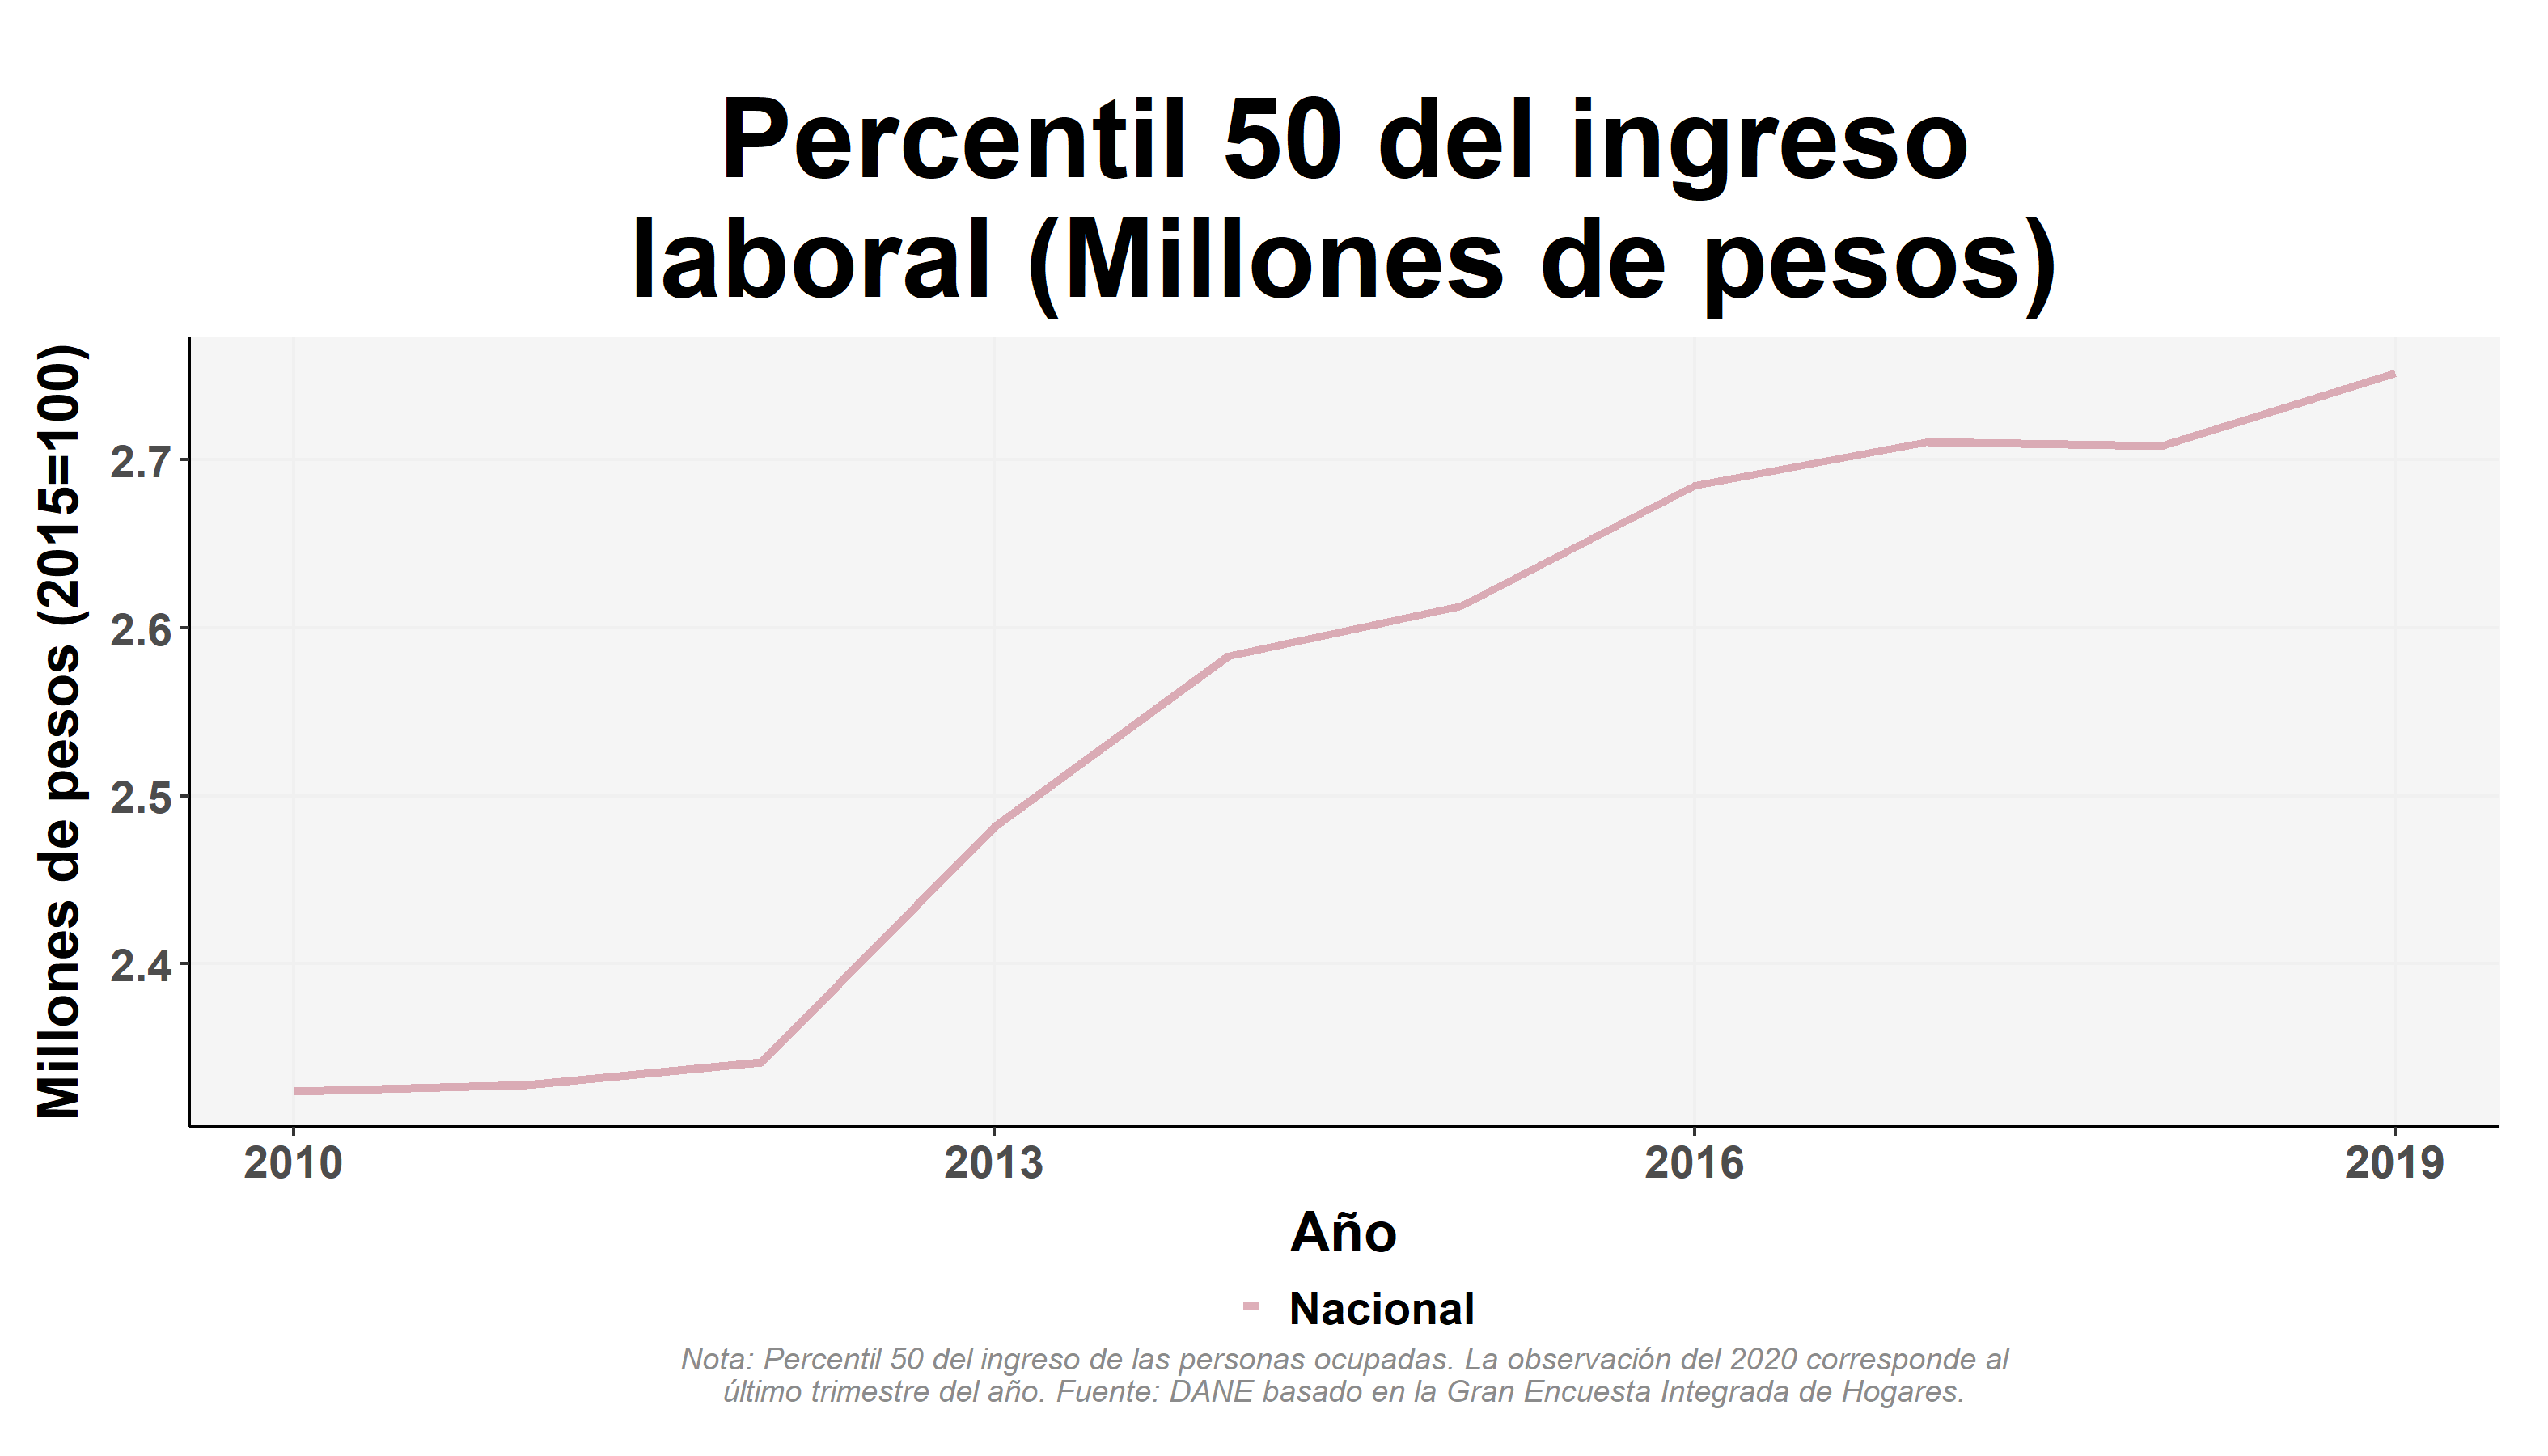
\includegraphics{img/var_17_trend.png}
            \end{imagecolumn}
            \begin{textcolumn}
                \begin{itemize}
                    \item El ingreso medio ha aumentado en los últimos años
                \end{itemize}
            \end{textcolumn}

    \printcolumns
    \end{slide}

    %%% Pctil 25 por genero
    \begin{slide}{3} 
                      \begin{imagecolumn}
                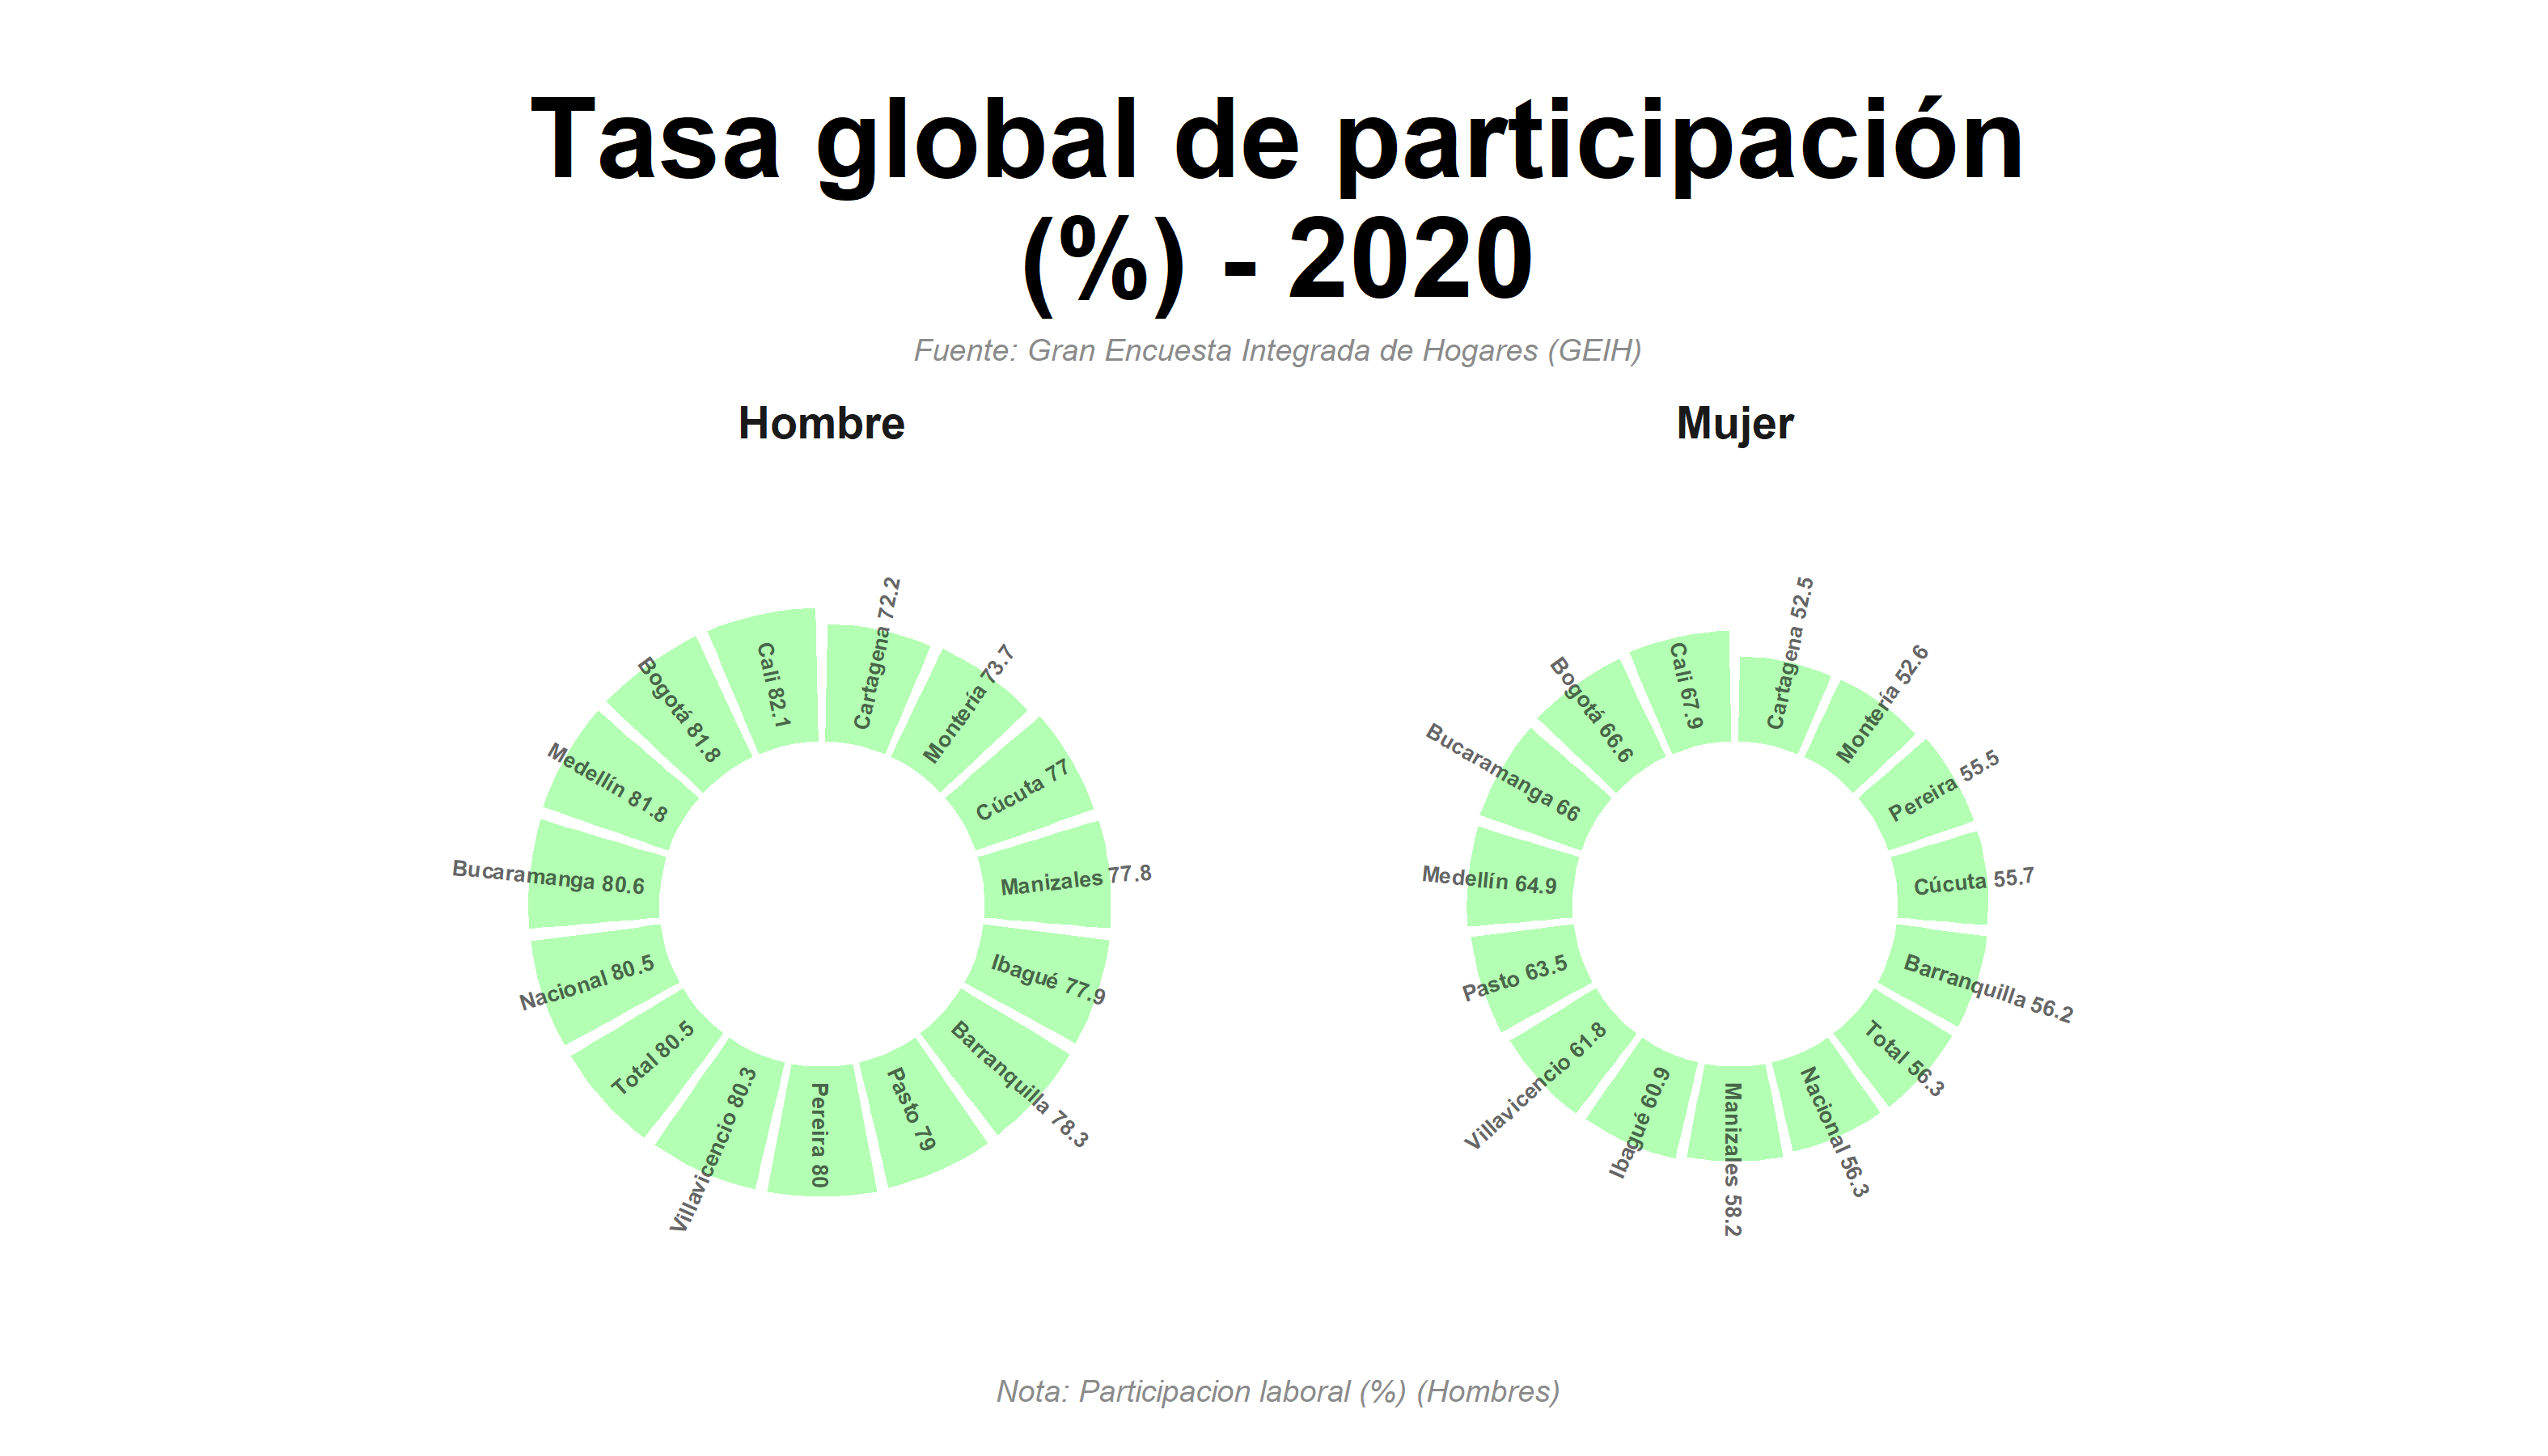
\includegraphics[width=\columnwidth]{img/var_102_static.png}
            \end{imagecolumn}
            \begin{textcolumn}
                \begin{itemize}
                    \item Pero hay una brecha de género enorme, especialmente en los percentiles más bajos de ingreso.
                    \item El rezago en el ingreso de las mujeres con respecto al de los hombres es de más de 10 años.
                \end{itemize}
            \end{textcolumn}

    \printcolumns
    \end{slide}

    
    %%% ----------------------------
    %%% Pobreza--
    %%% ----------------------------
    \subsection{Pobreza}
    
        %%%-- Highlights 
    \begin{slide}{4} 
                      \begin{imagecolumn}
                \includegraphics[width=\columnwidth]{img/var_369_map.png}
            \end{imagecolumn}
            \begin{textcolumn}
                \begin{itemize}
                    \item A nivel nacional, existe una tendencia a la baja de la pobreza no monetaria
                    \item No obstante, las brechas territoriales son grandes y persisten.
                \end{itemize}
            \end{textcolumn}

    \printcolumns
    \end{slide}
     
    
    %%% Interiores
    \begin{slide}{4} 
            \begin{imagecolumn}
                \includegraphics[width=\columnwidth]{img/var_362_scatter_time.png}
            \end{imagecolumn}
            \begin{textcolumn}
                \begin{itemize}
                    \item Esta misma tendencia se mantiene en la pobreza monetaria
                \end{itemize}
            \end{textcolumn}

    \printcolumns
    \end{slide}
    
        %%% Interiores
    \begin{slide}{4} 
            \begin{imagecolumn}
                \includegraphics[width=\columnwidth]{img/var_364_trend.png}
            \end{imagecolumn}
            \begin{textcolumn}
                \begin{itemize}
                    \item La pandemia generó convergencia entre zonas urbanas y rurales, por el drástico aumento de la pobreza en las ciudades.
                \end{itemize}
            \end{textcolumn}

    \printcolumns
    \end{slide}
    
    
    %%% ----------------------------
    %%% Desigualdad--
    %%% ----------------------------
    \subsection{Desigualdad}
 
     %%% Gini zonas
    \begin{slide}{5} 
            \begin{imagecolumn}
                \includegraphics[width=\columnwidth]{img/var_354_trend.png}
            \end{imagecolumn}
            \begin{textcolumn}
                \begin{itemize}
                    \item Hasta 2017 la desigualdad venia disminuyendo en todas las zonas, pero la pandemia devolvió a los territorios a los niveles de desigualdad de hace 10 años.
                \end{itemize}
            \end{textcolumn}

    \printcolumns
    \end{slide}
    
        %%%-- Gini departamentos 
    \begin{slide}{5} 
                      \begin{imagecolumn}
                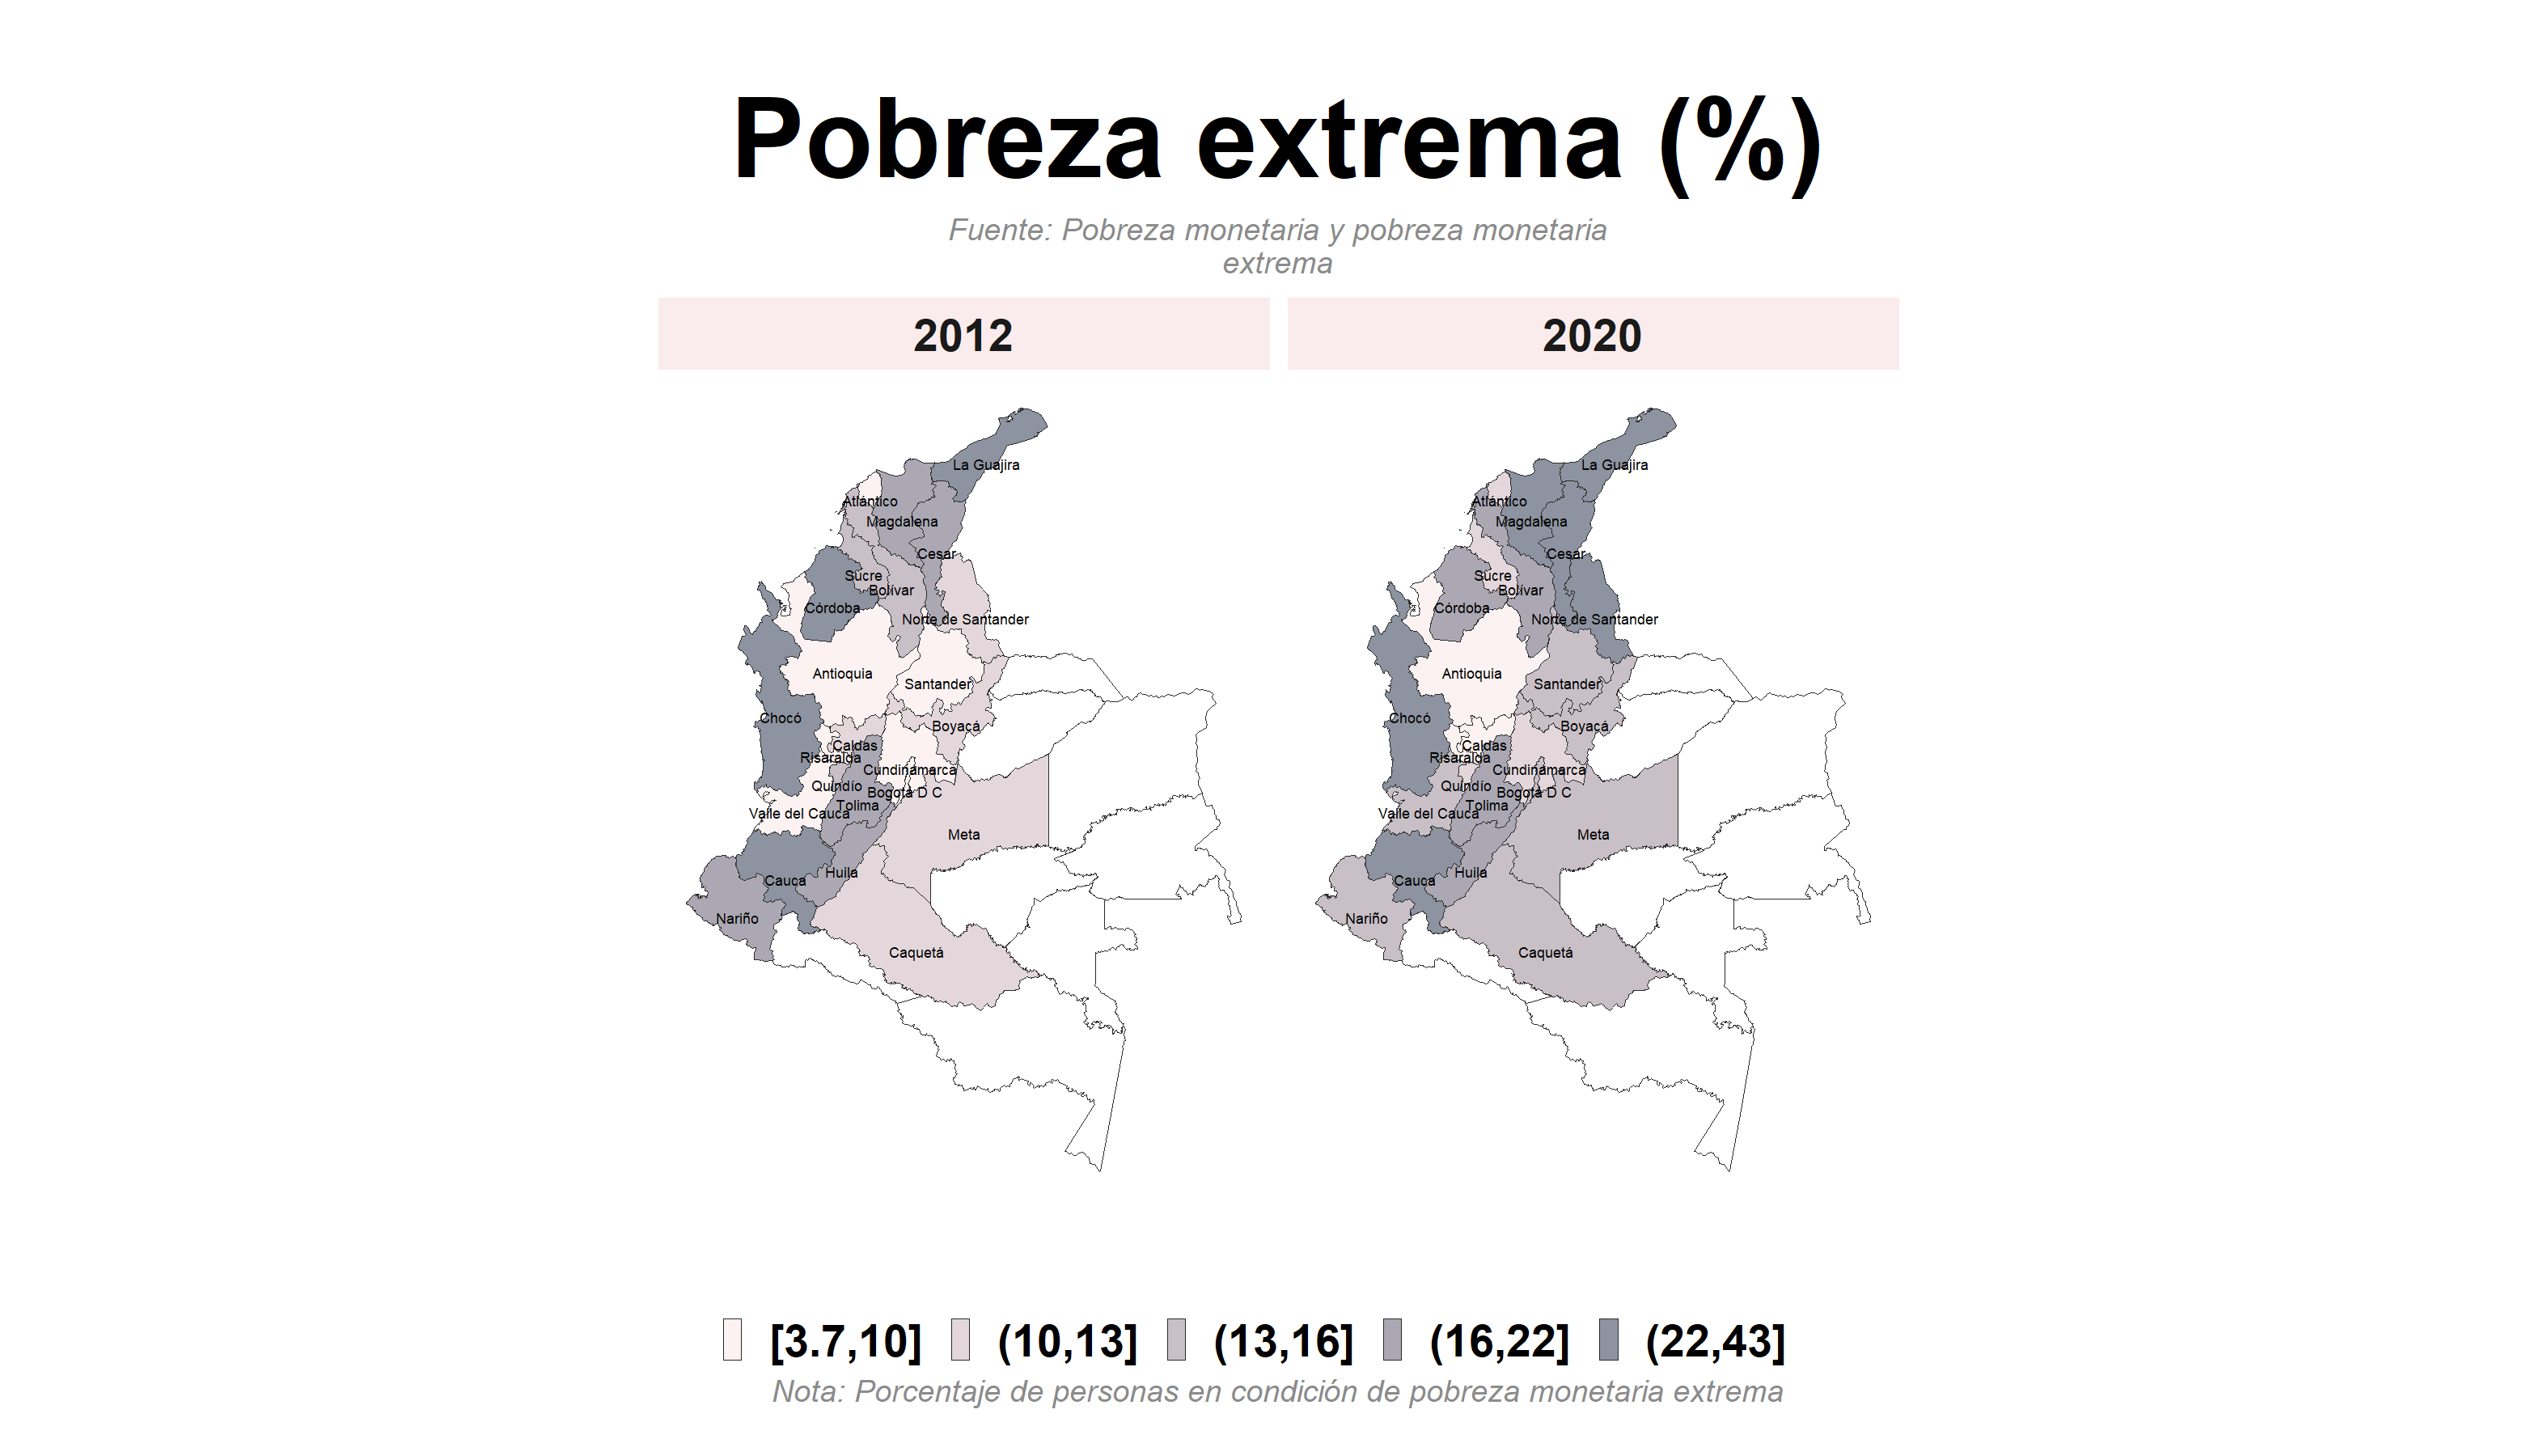
\includegraphics[width=\columnwidth]{img/var_288_map.png}
            \end{imagecolumn}
            \begin{textcolumn}
                \begin{itemize}
                    \item Aún así, comparado con 2002 la desigualdad ha disminuido en muchos territorios
                    \item Pero algunos departamentos como Chocó y La Guajira persisten en sus niveles de desigualdad de hace 20 años.
                \end{itemize}
            \end{textcolumn}

    \printcolumns
    \end{slide}
     
    

    
    %%% ----------------------------
    %%% Caractirísticas del hogar
    %%% ----------------------------
    \subsection{Característica del hogar}
    
        %%%-- Hacinamiento Crítico 
    \begin{slide}{6} 
                      \begin{imagecolumn}
                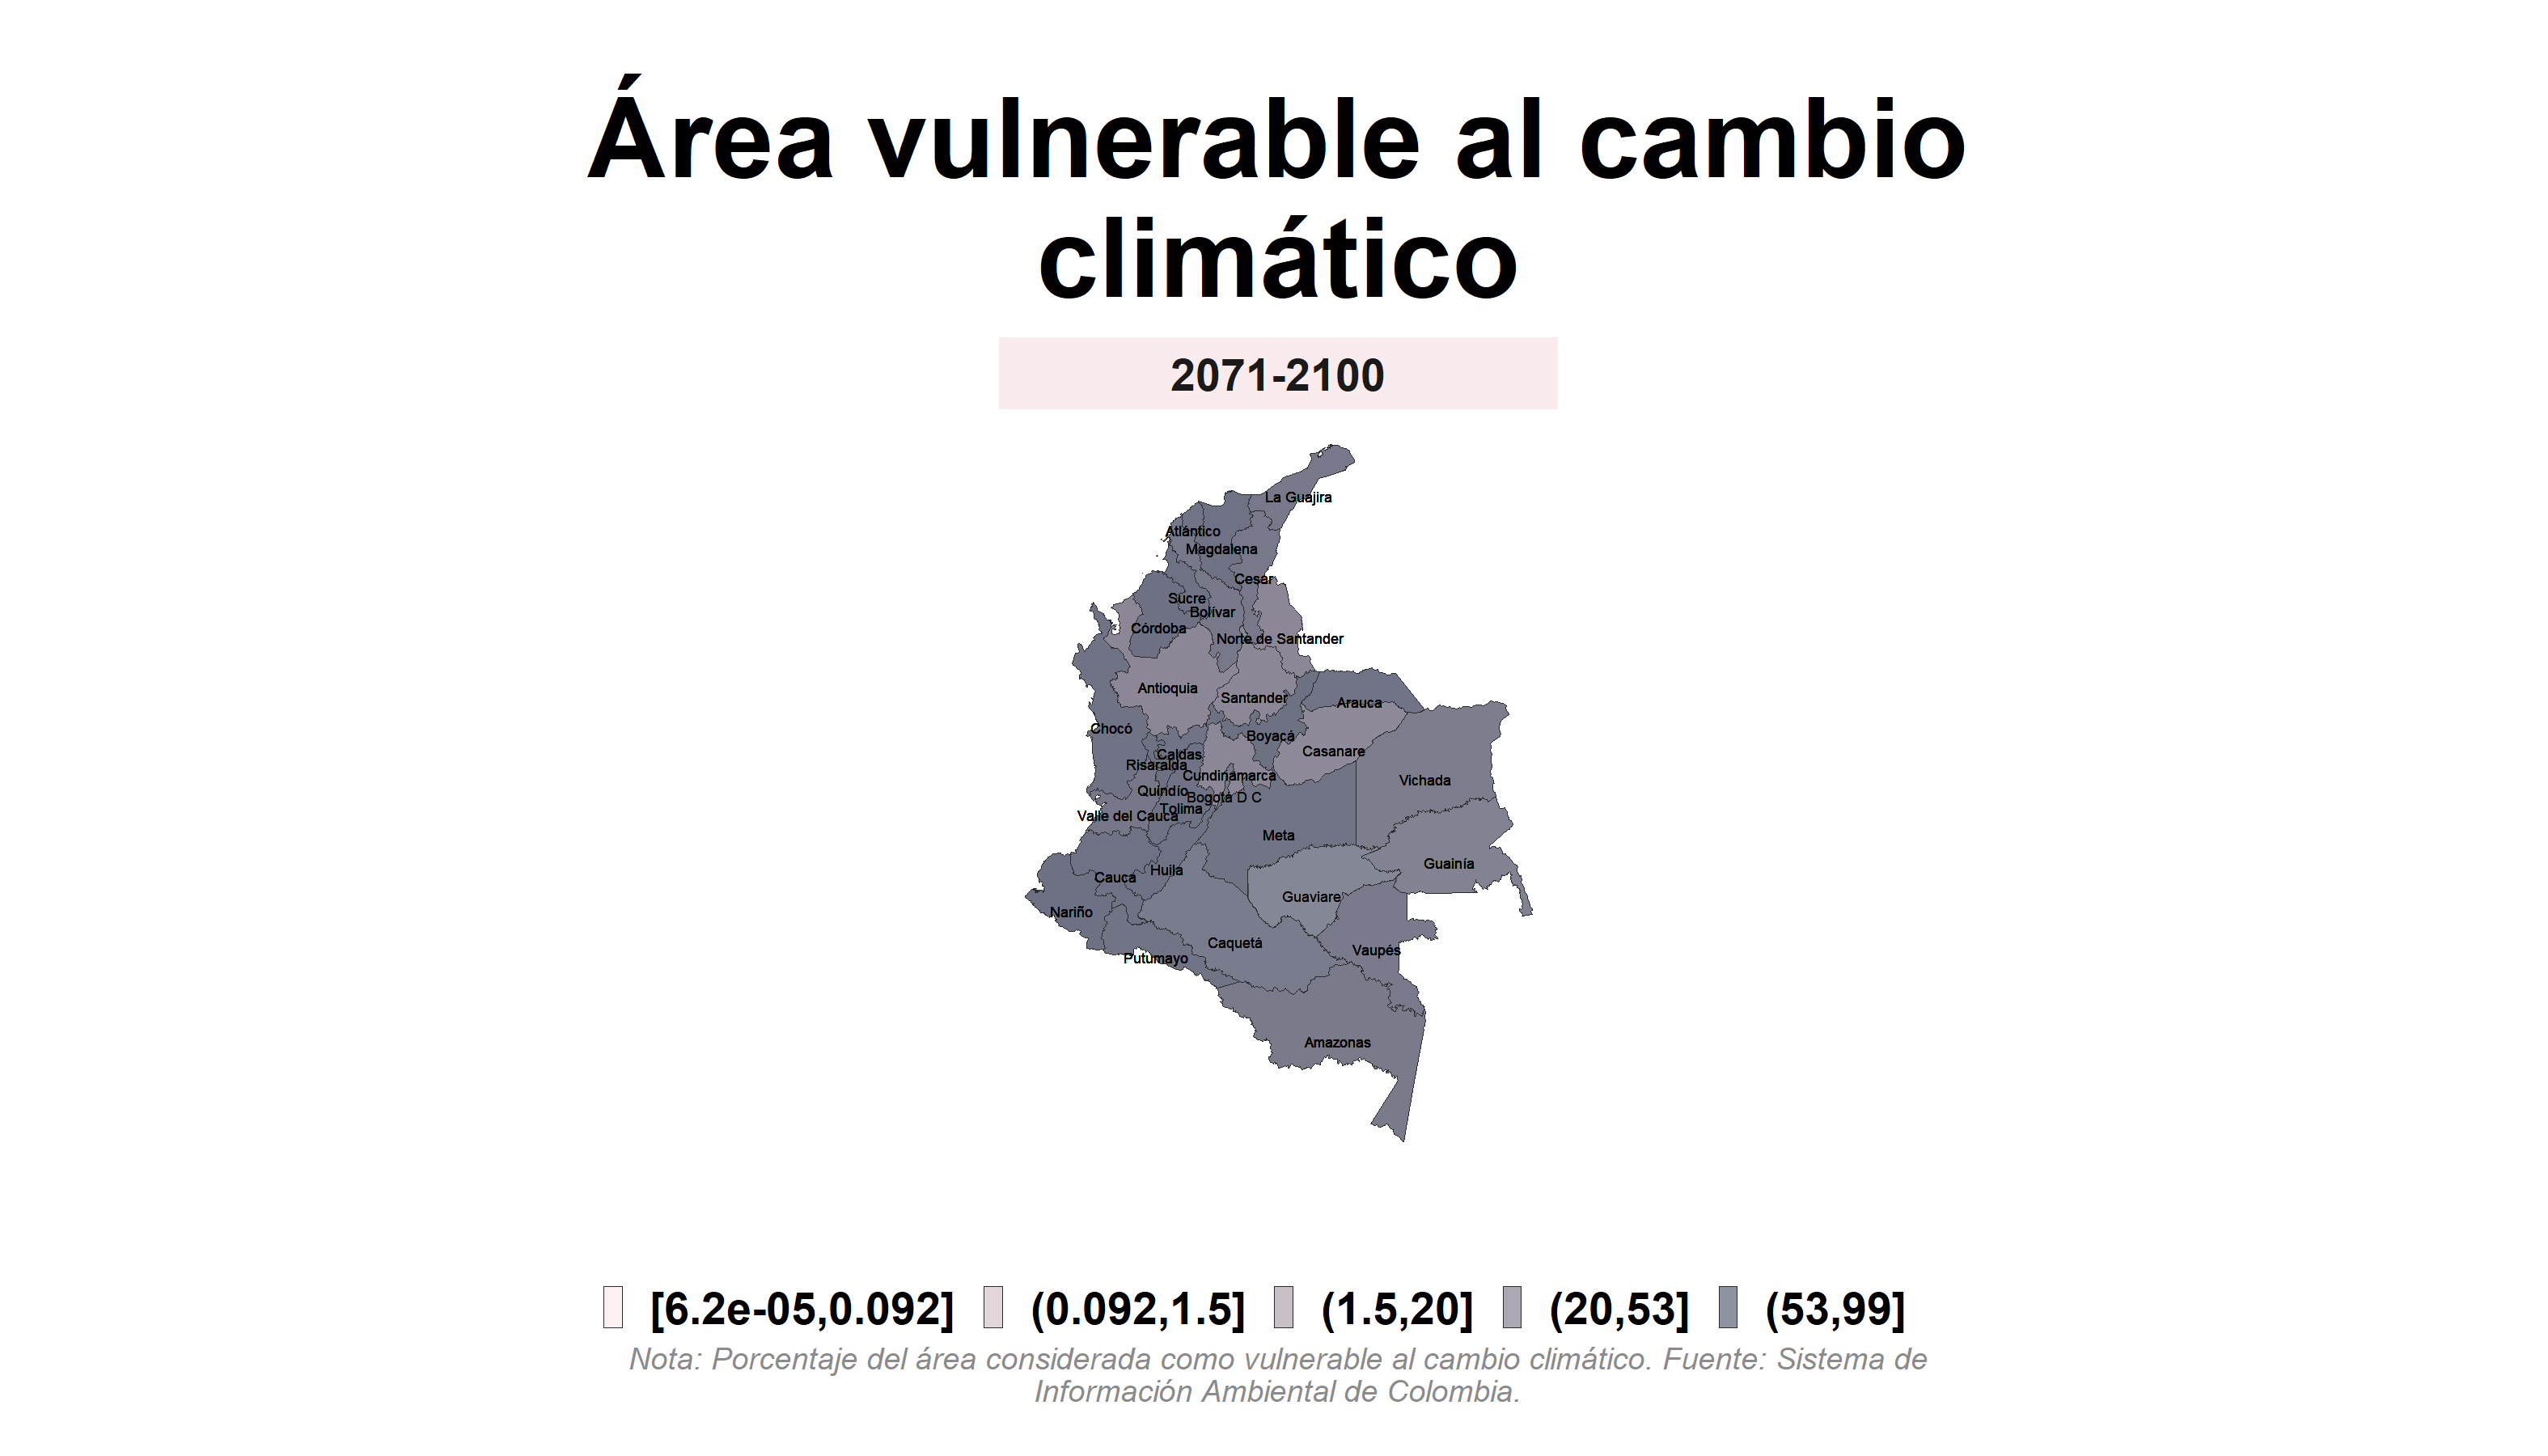
\includegraphics[width=\columnwidth]{img/var_299_map.png}
            \end{imagecolumn}
            \begin{textcolumn}
                \begin{itemize}
                    \item Existe una alta variación en el hacinamiento crítico entre regiones 
                    \item Esto puede estar asociado a las estructuras étnicas en algunos departamentos
                \end{itemize}
            \end{textcolumn}

    \printcolumns
    \end{slide}
    
    
        
    %%% ----------------------------
    %%% Acceso a Agua Potable
    %%% ----------------------------
    \subsection{Acceso a servicios de Agua Potable}
    
        %%%-- Highlights 
    \begin{slide}{7} 
                      \begin{imagecolumn}
                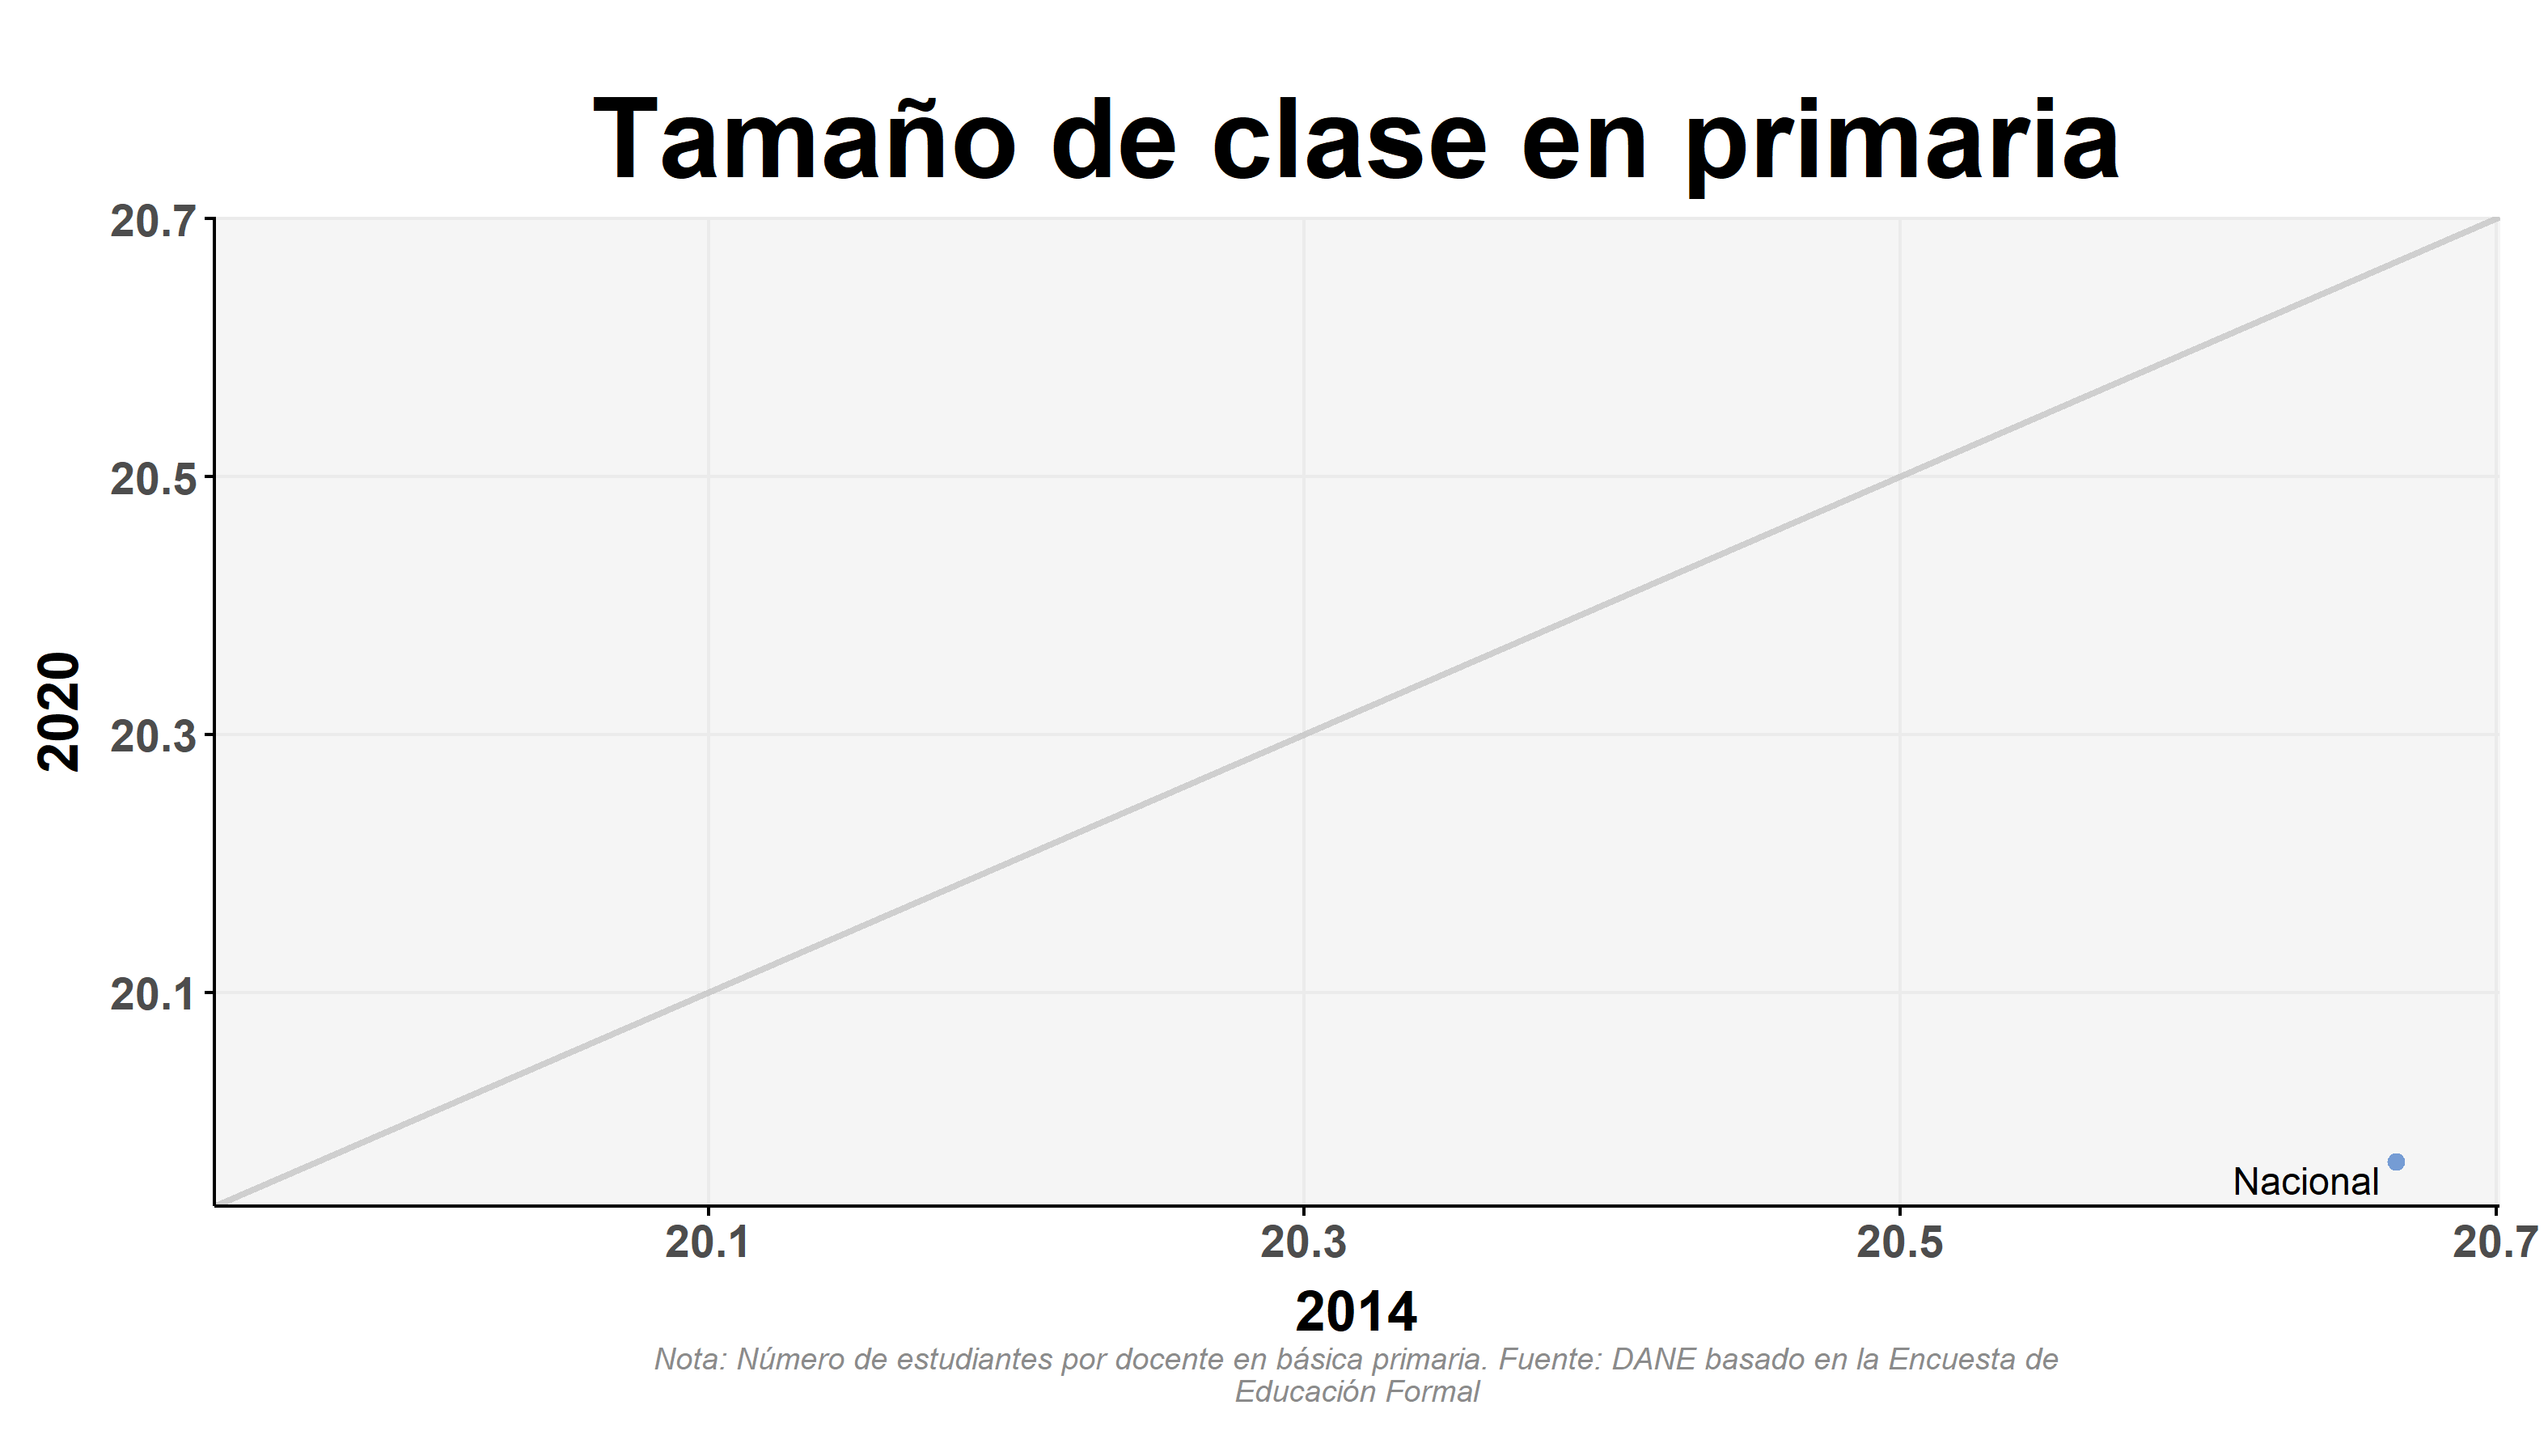
\includegraphics[width=\columnwidth]{img/var_229_scatter_time.png}
            \end{imagecolumn}
            \begin{textcolumn}
                \begin{itemize}
                    \item Aunque en promedio existe una mejora en el acceso a saneamiento básico, en algunos departamentos como Amazonas, Putumayo y Arauca el saneamiento ha desmejorado. 
                \end{itemize}
            \end{textcolumn}

    \printcolumns
    \end{slide}
    
    
    %%% ----------------------------
    %%% Caractirísticas del hogar
    %%% ----------------------------
    \subsection{Crecimiento Económico}
    
        %%%-- Highlights 
    \begin{slide}{8} 
                      \begin{imagecolumn}
                \includegraphics[width=\columnwidth]{img/var_334_map.png}
            \end{imagecolumn}
            \begin{textcolumn}
                \begin{itemize}
                    \item Las regiones son ahora más diversas en términos de actividad económica.
                    \item Pero en los departamentos más marginados persiste una alta dependencia de ciertos sectores
                \end{itemize}
            \end{textcolumn}

    \printcolumns
    \end{slide}
    
    
            %%%-- Highlights 
    \begin{slide}{8} 
            \begin{imagecolumn}
                \includegraphics[width=\columnwidth]{img/var_335_static.png}
            \end{imagecolumn}
            \begin{textcolumn}
                \begin{itemize}
                    \item El índice de luminosidad confirma la heterogeneidad en actividad económica entre regiones.
                \end{itemize}
            \end{textcolumn}

    \printcolumns
    \end{slide}
    
    
    %%% ----------------------------
    %%% Migracion
    %%% ----------------------------
    \subsection{Migración}
    
        %%%-- Highlights 
    \begin{slide}{10} 
                      \begin{imagecolumn}
                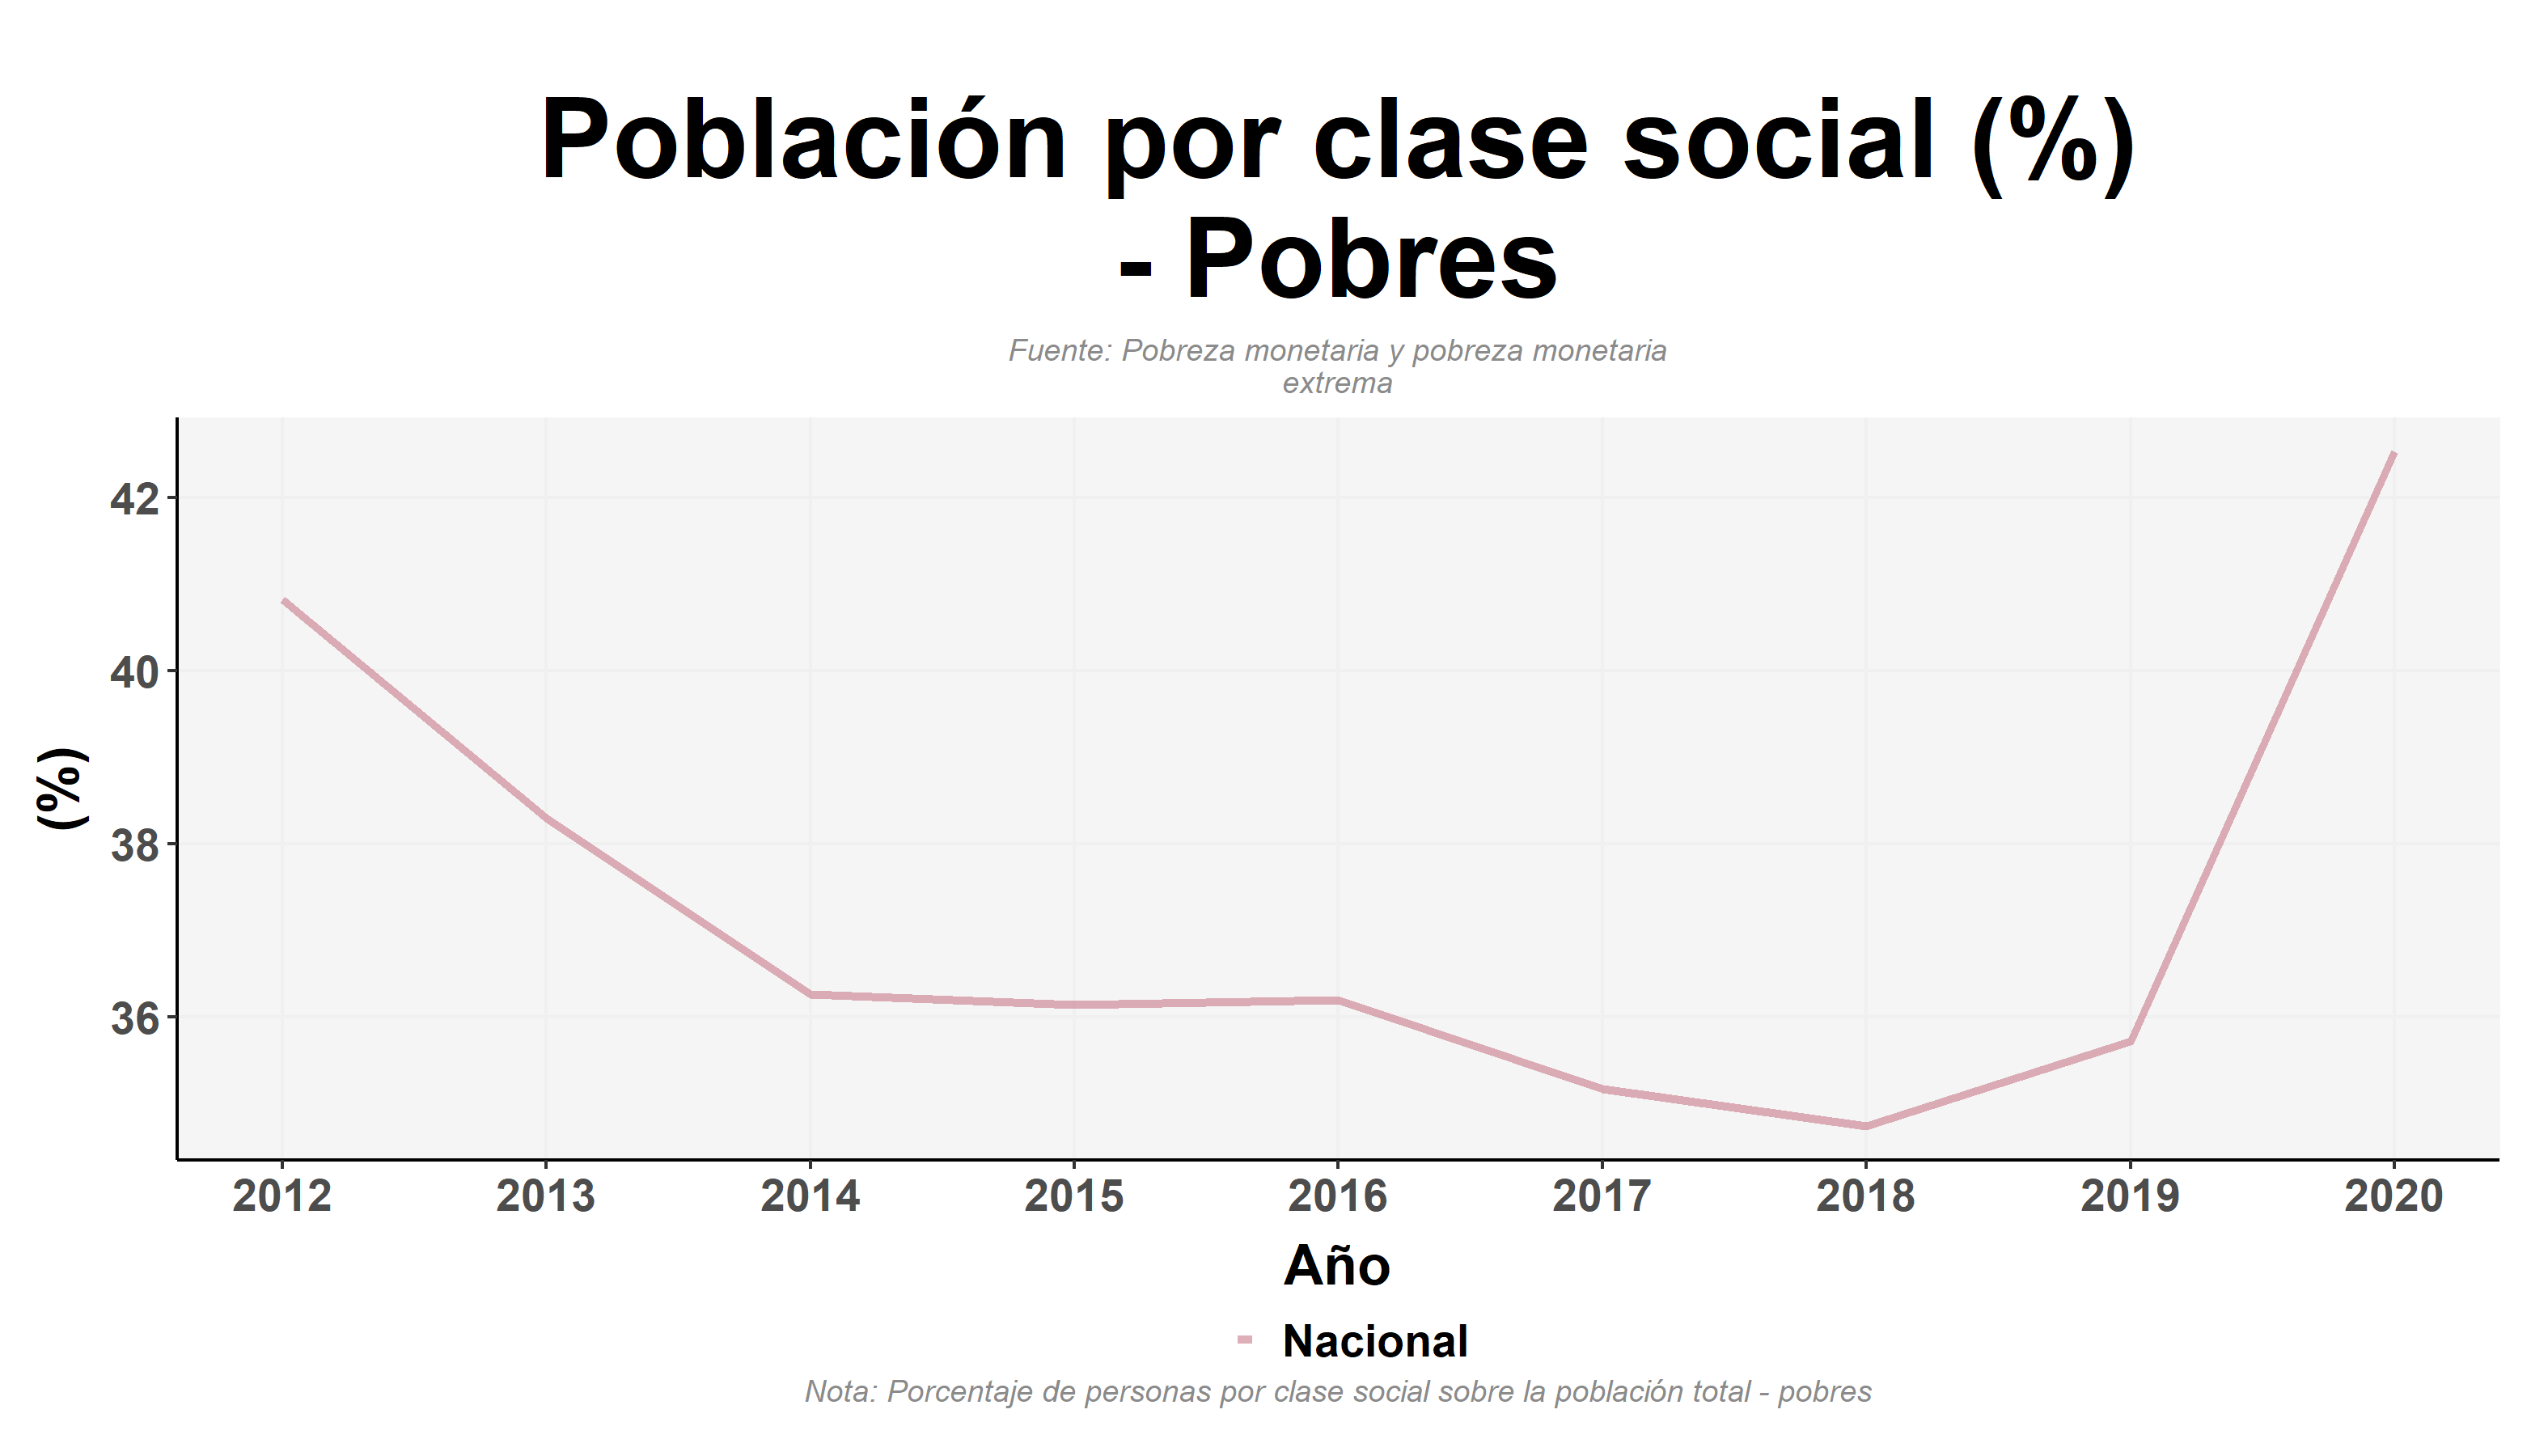
\includegraphics[width=\columnwidth]{img/var_272_trend.png}
            \end{imagecolumn}
            \begin{textcolumn}
                \begin{itemize}
                    \item La crisis migratoria venezolana se concentró en el grupo de edad entre los 16-55 años.
                \end{itemize}
            \end{textcolumn}

    \printcolumns
    \end{slide}
    
    %%% ----------------------------
    %%% Cambio Climático
    %%% ----------------------------
    \subsection{Cambio Climático}
    
        %%%-- Highlights 
    \begin{slide}{11} 
                      \begin{imagecolumn}
                \includegraphics[width=\columnwidth]{img/var_333_map.png}
            \end{imagecolumn}
            \begin{textcolumn}
                \begin{itemize}
                    \item El impacto del cambio climático tendrá efectos diferenciados en las regiones del país
                \end{itemize}
            \end{textcolumn}

    \printcolumns
    \end{slide}
    
        %%% ----------------------------
    %%% Indicadores de resutlados
    %%% ----------------------------
    
     \section{Resultados}
    %%% Contexto
    \slidetitle{12}
    
        %%% ----------------------------
    %%% Infancia y Niñez
    %%% ----------------------------
    \subsection{Infancia y niñez}
    
        %%%-- Tasa de Mortalidad Infantil 
    \begin{slide}{13} 
                      \begin{imagecolumn}
                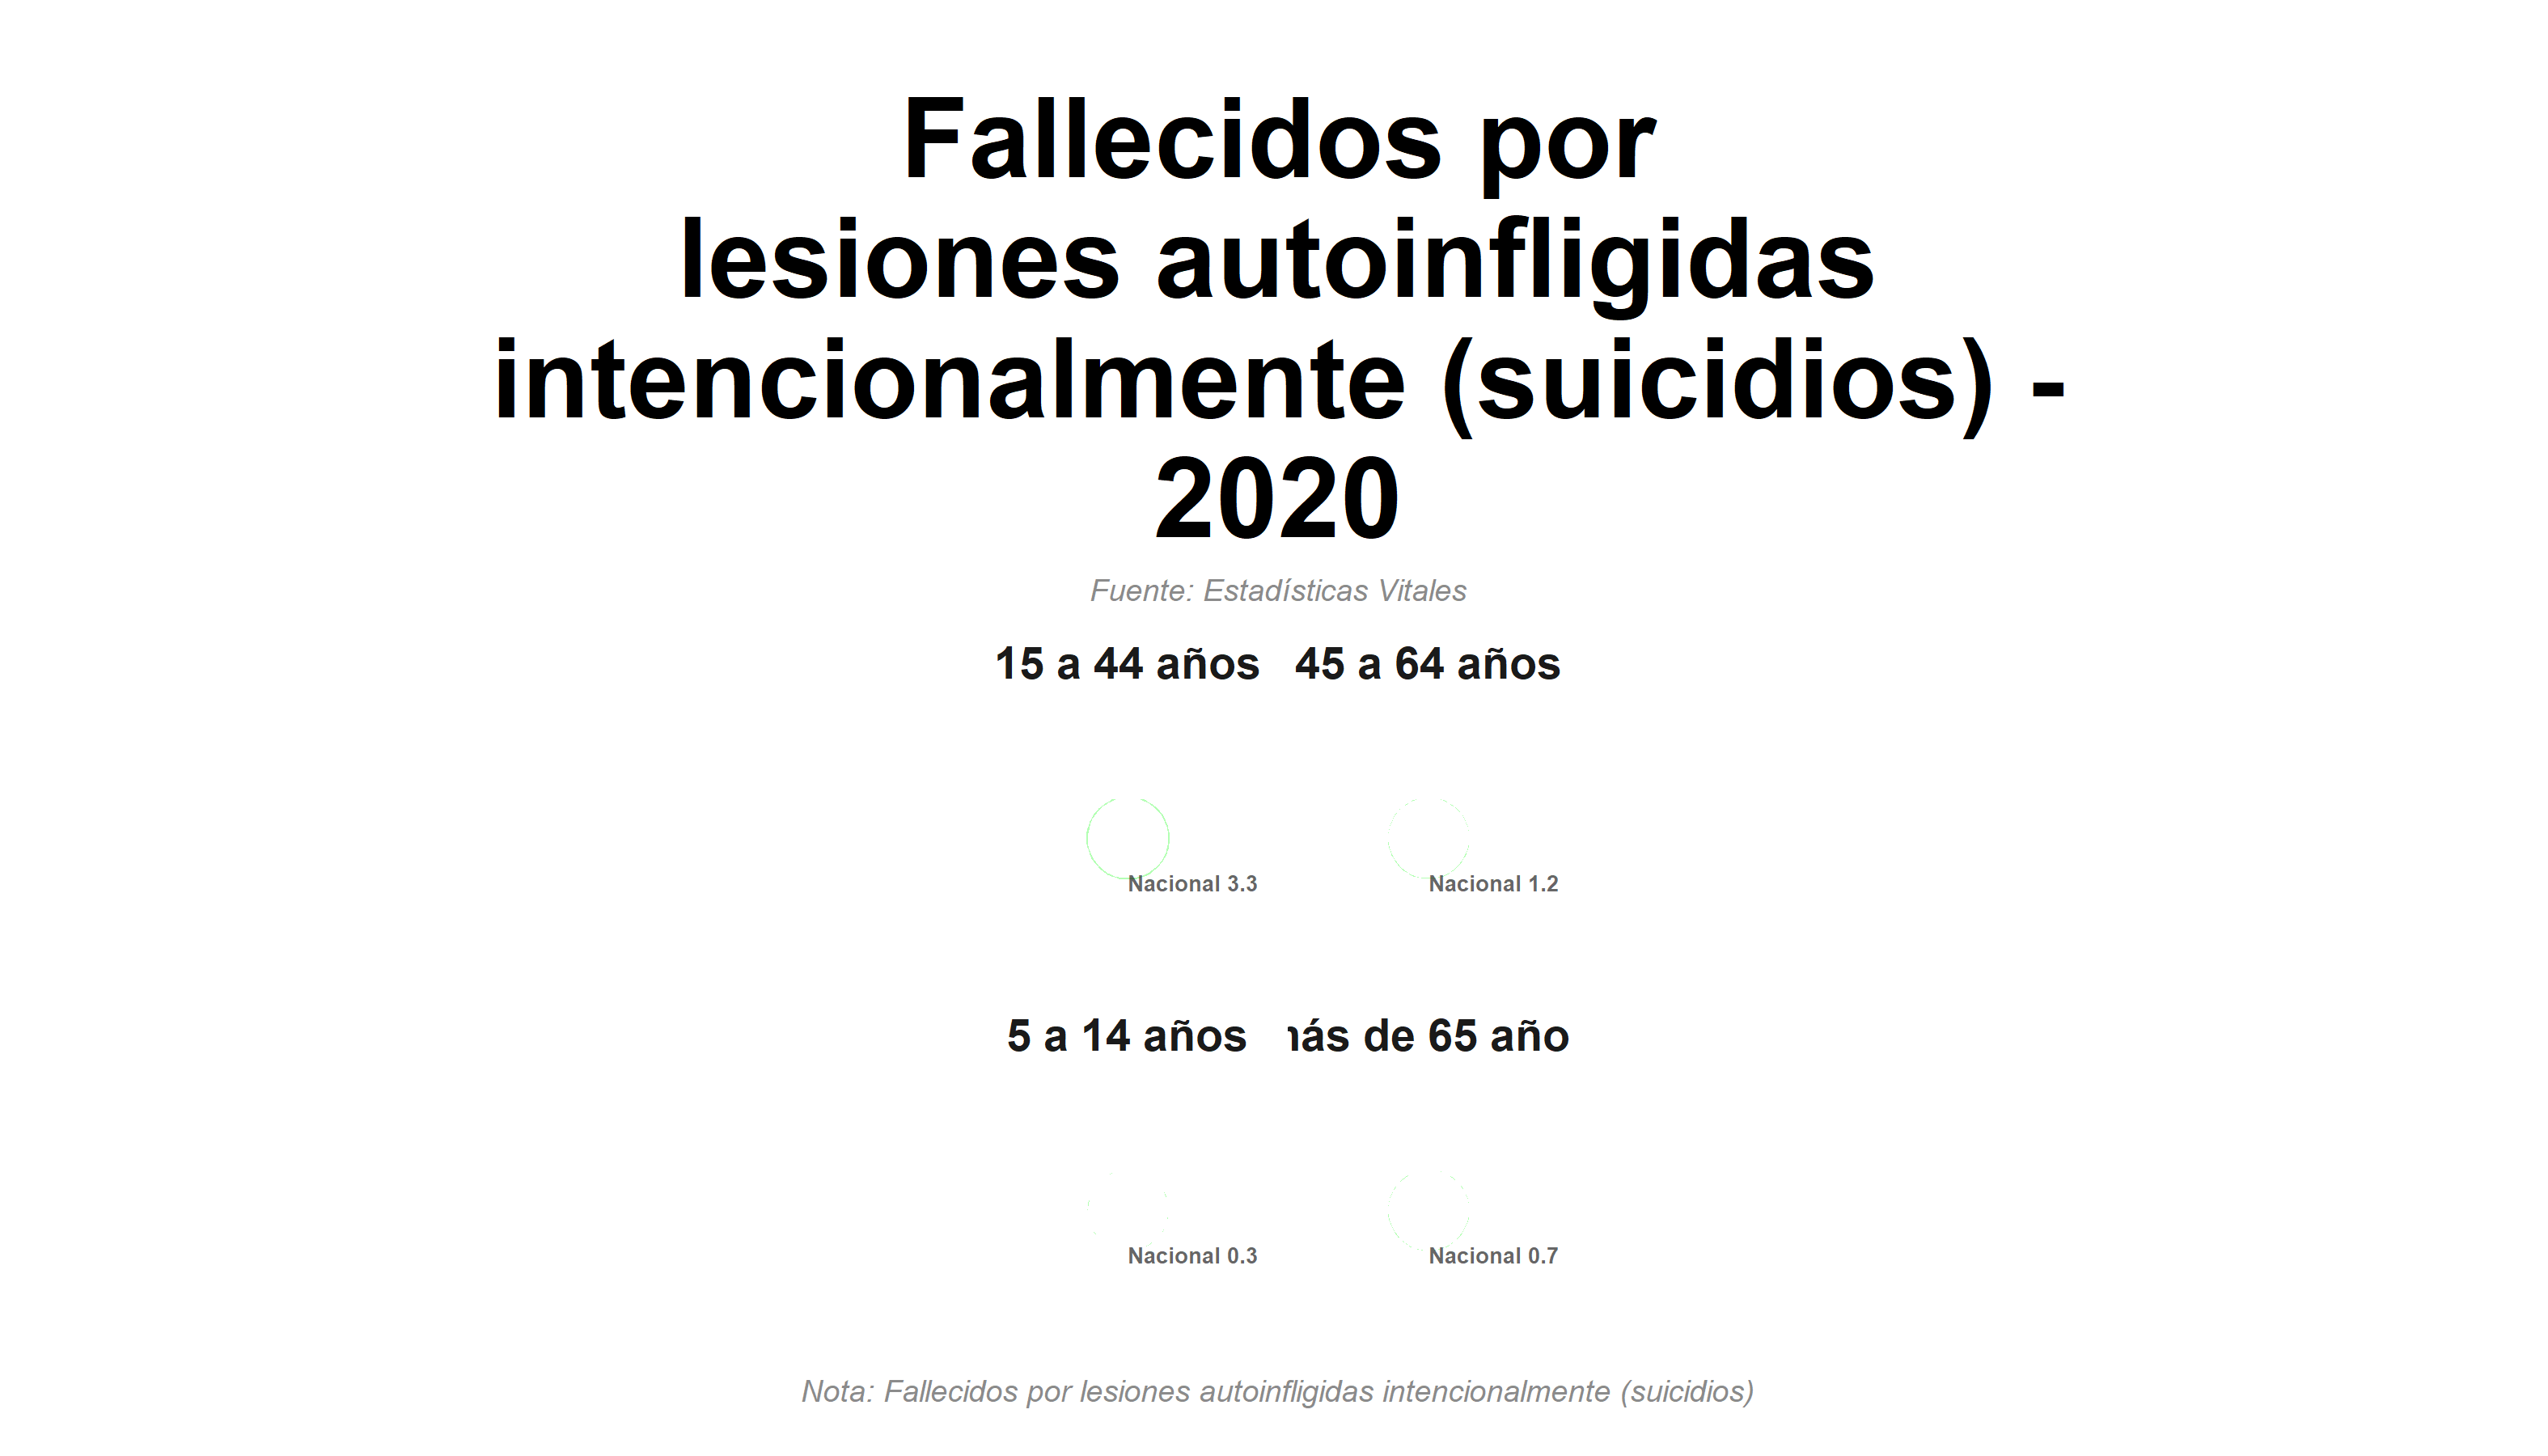
\includegraphics[width=\columnwidth]{img/var_325_static.png}
            \end{imagecolumn}
            \begin{textcolumn}
                \begin{itemize}
                    \item En Colombia coexisten regiones con tasas de mortalidad infantil similares a las de Sur Africa (24%, Vichada) y a las de Estados Unidos (6%, Boyacá)
                \end{itemize}
            \end{textcolumn}

    \printcolumns
    \end{slide}
    
        \begin{slide}{13} 
                      \begin{imagecolumn}
                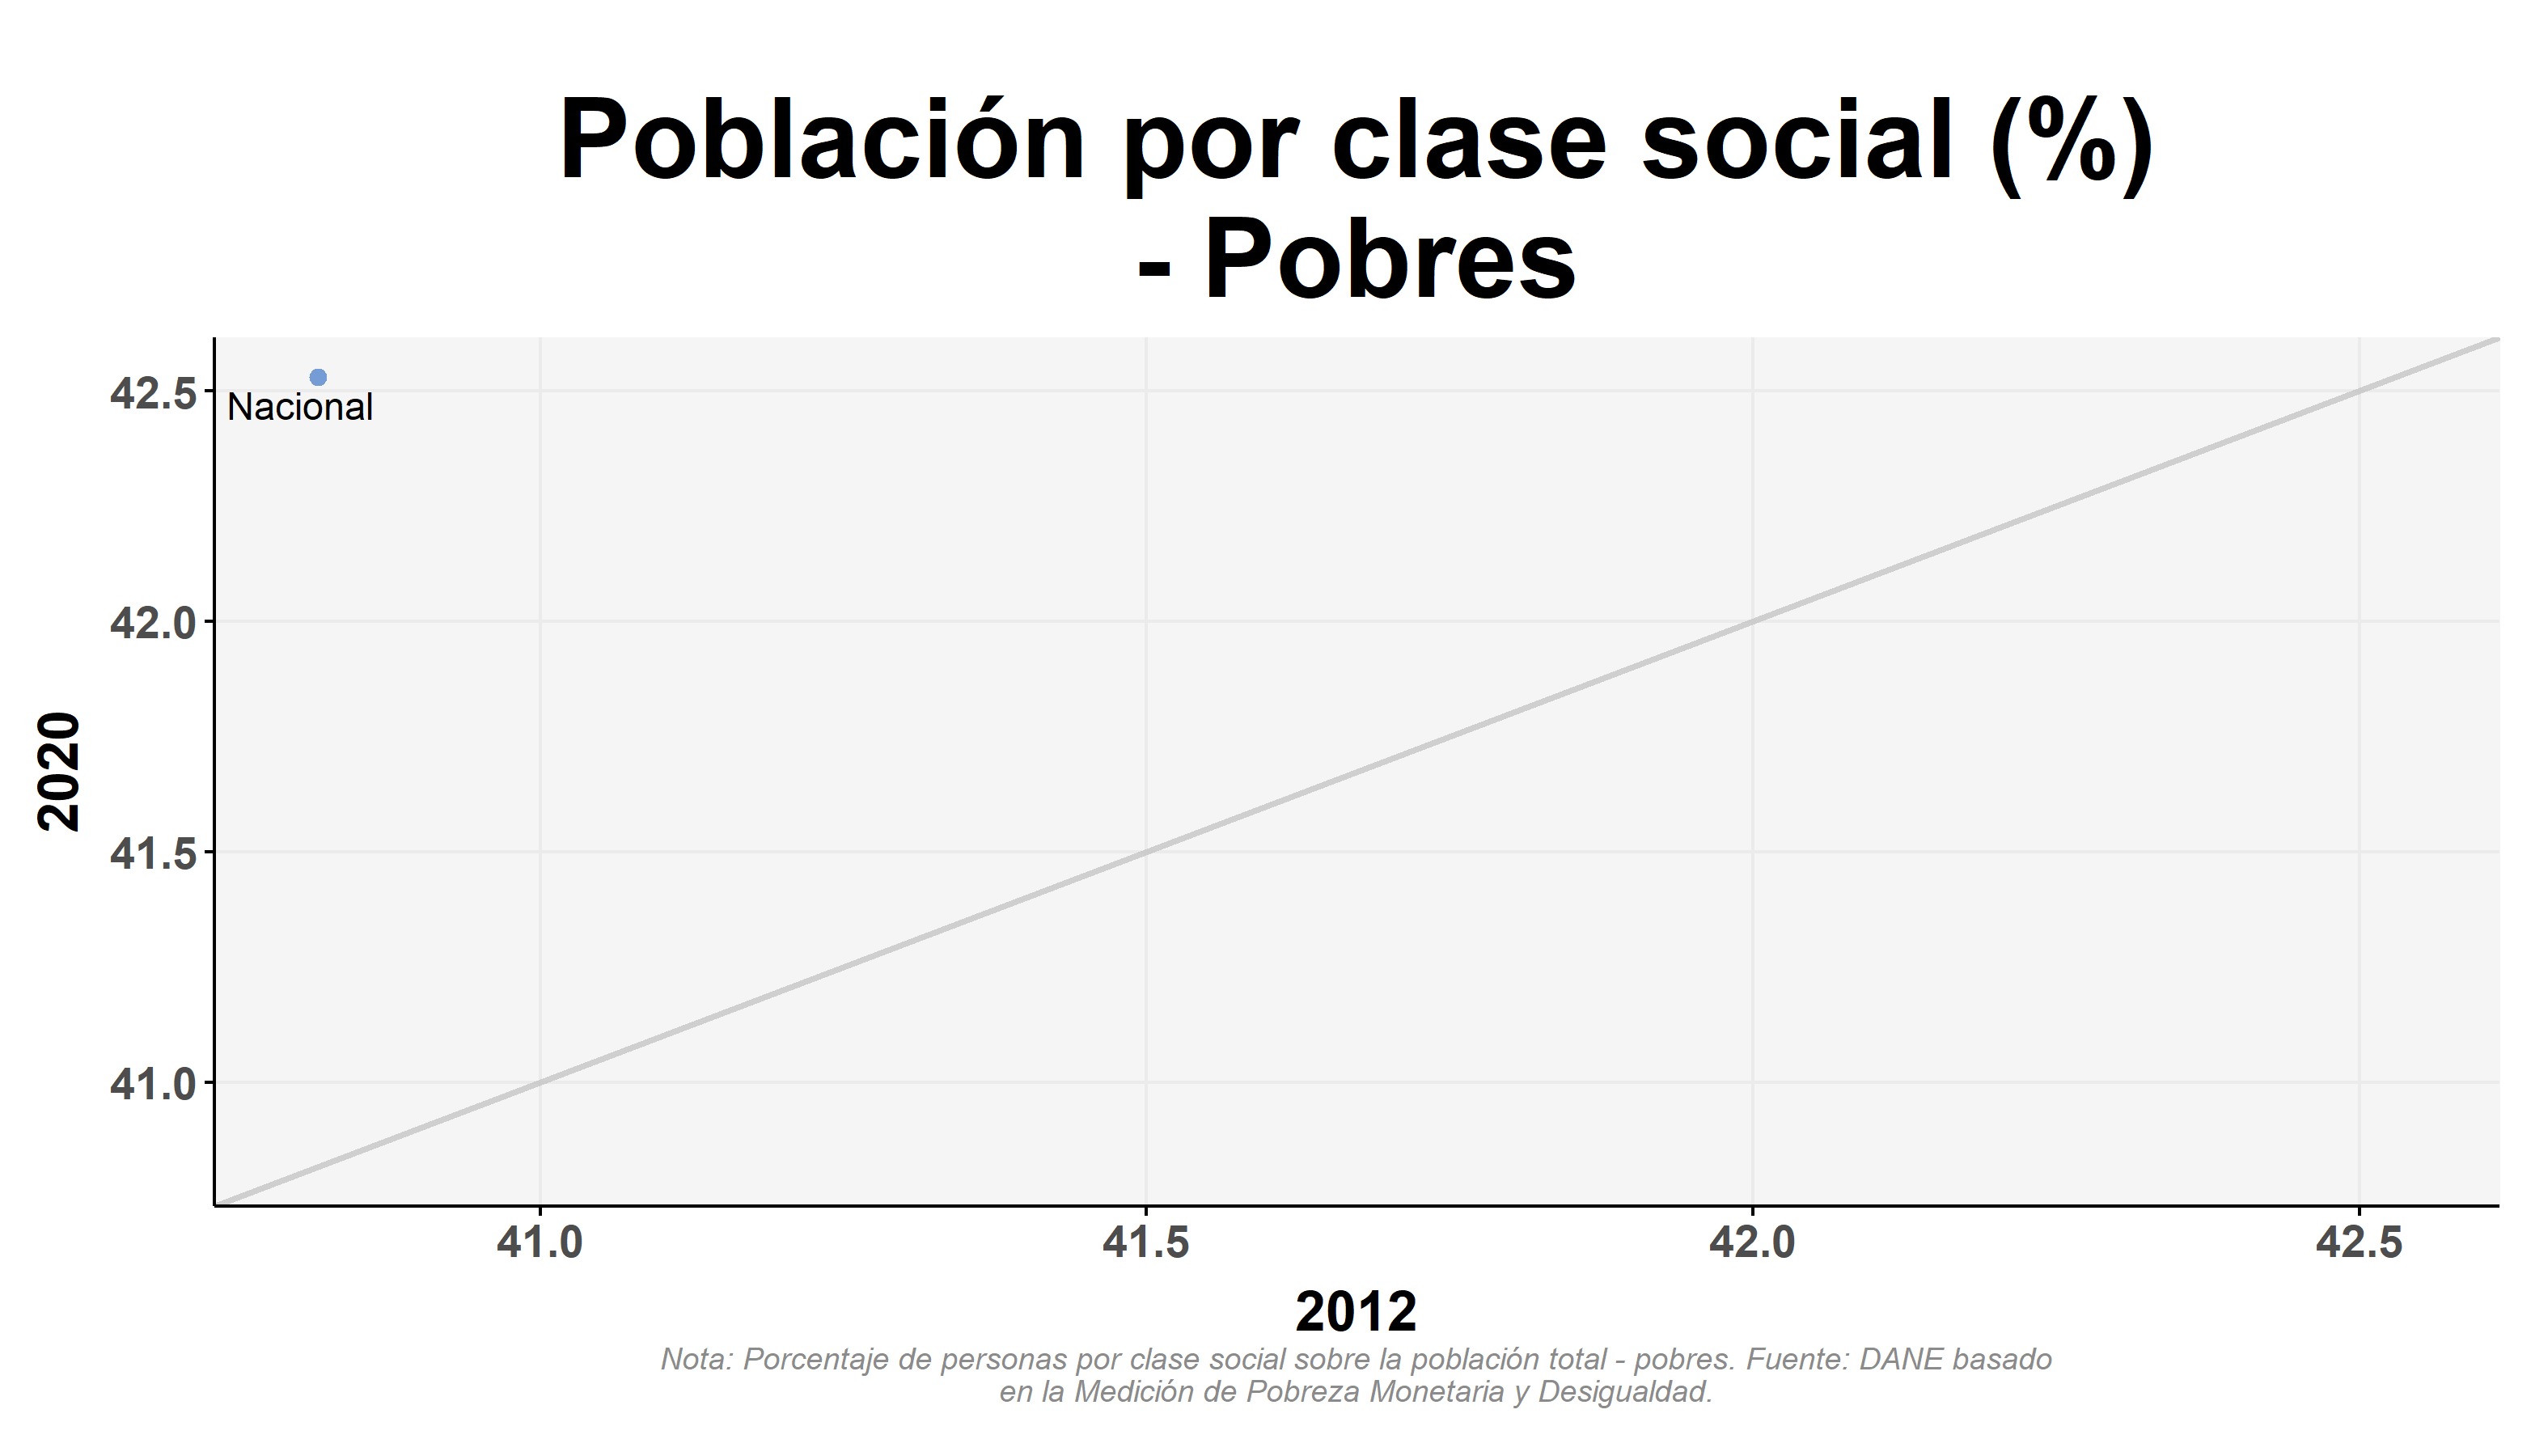
\includegraphics[width=\columnwidth]{img/var_242_scatter_time.png}
            \end{imagecolumn}
            \begin{textcolumn}
                \begin{itemize}
                    \item En la mayor parte de las regiones, la mortalidad infantil disminuyó entre 2005 y 2015. 
                    \item Pero en departamentos como Guajira y Vaupés, ésta tasa aumentó.
                \end{itemize}
            \end{textcolumn}

    \printcolumns
    \end{slide}
  
      %%%-- Tamaño de clase 
  
            \begin{slide}{13} 
                      \begin{imagecolumn}
                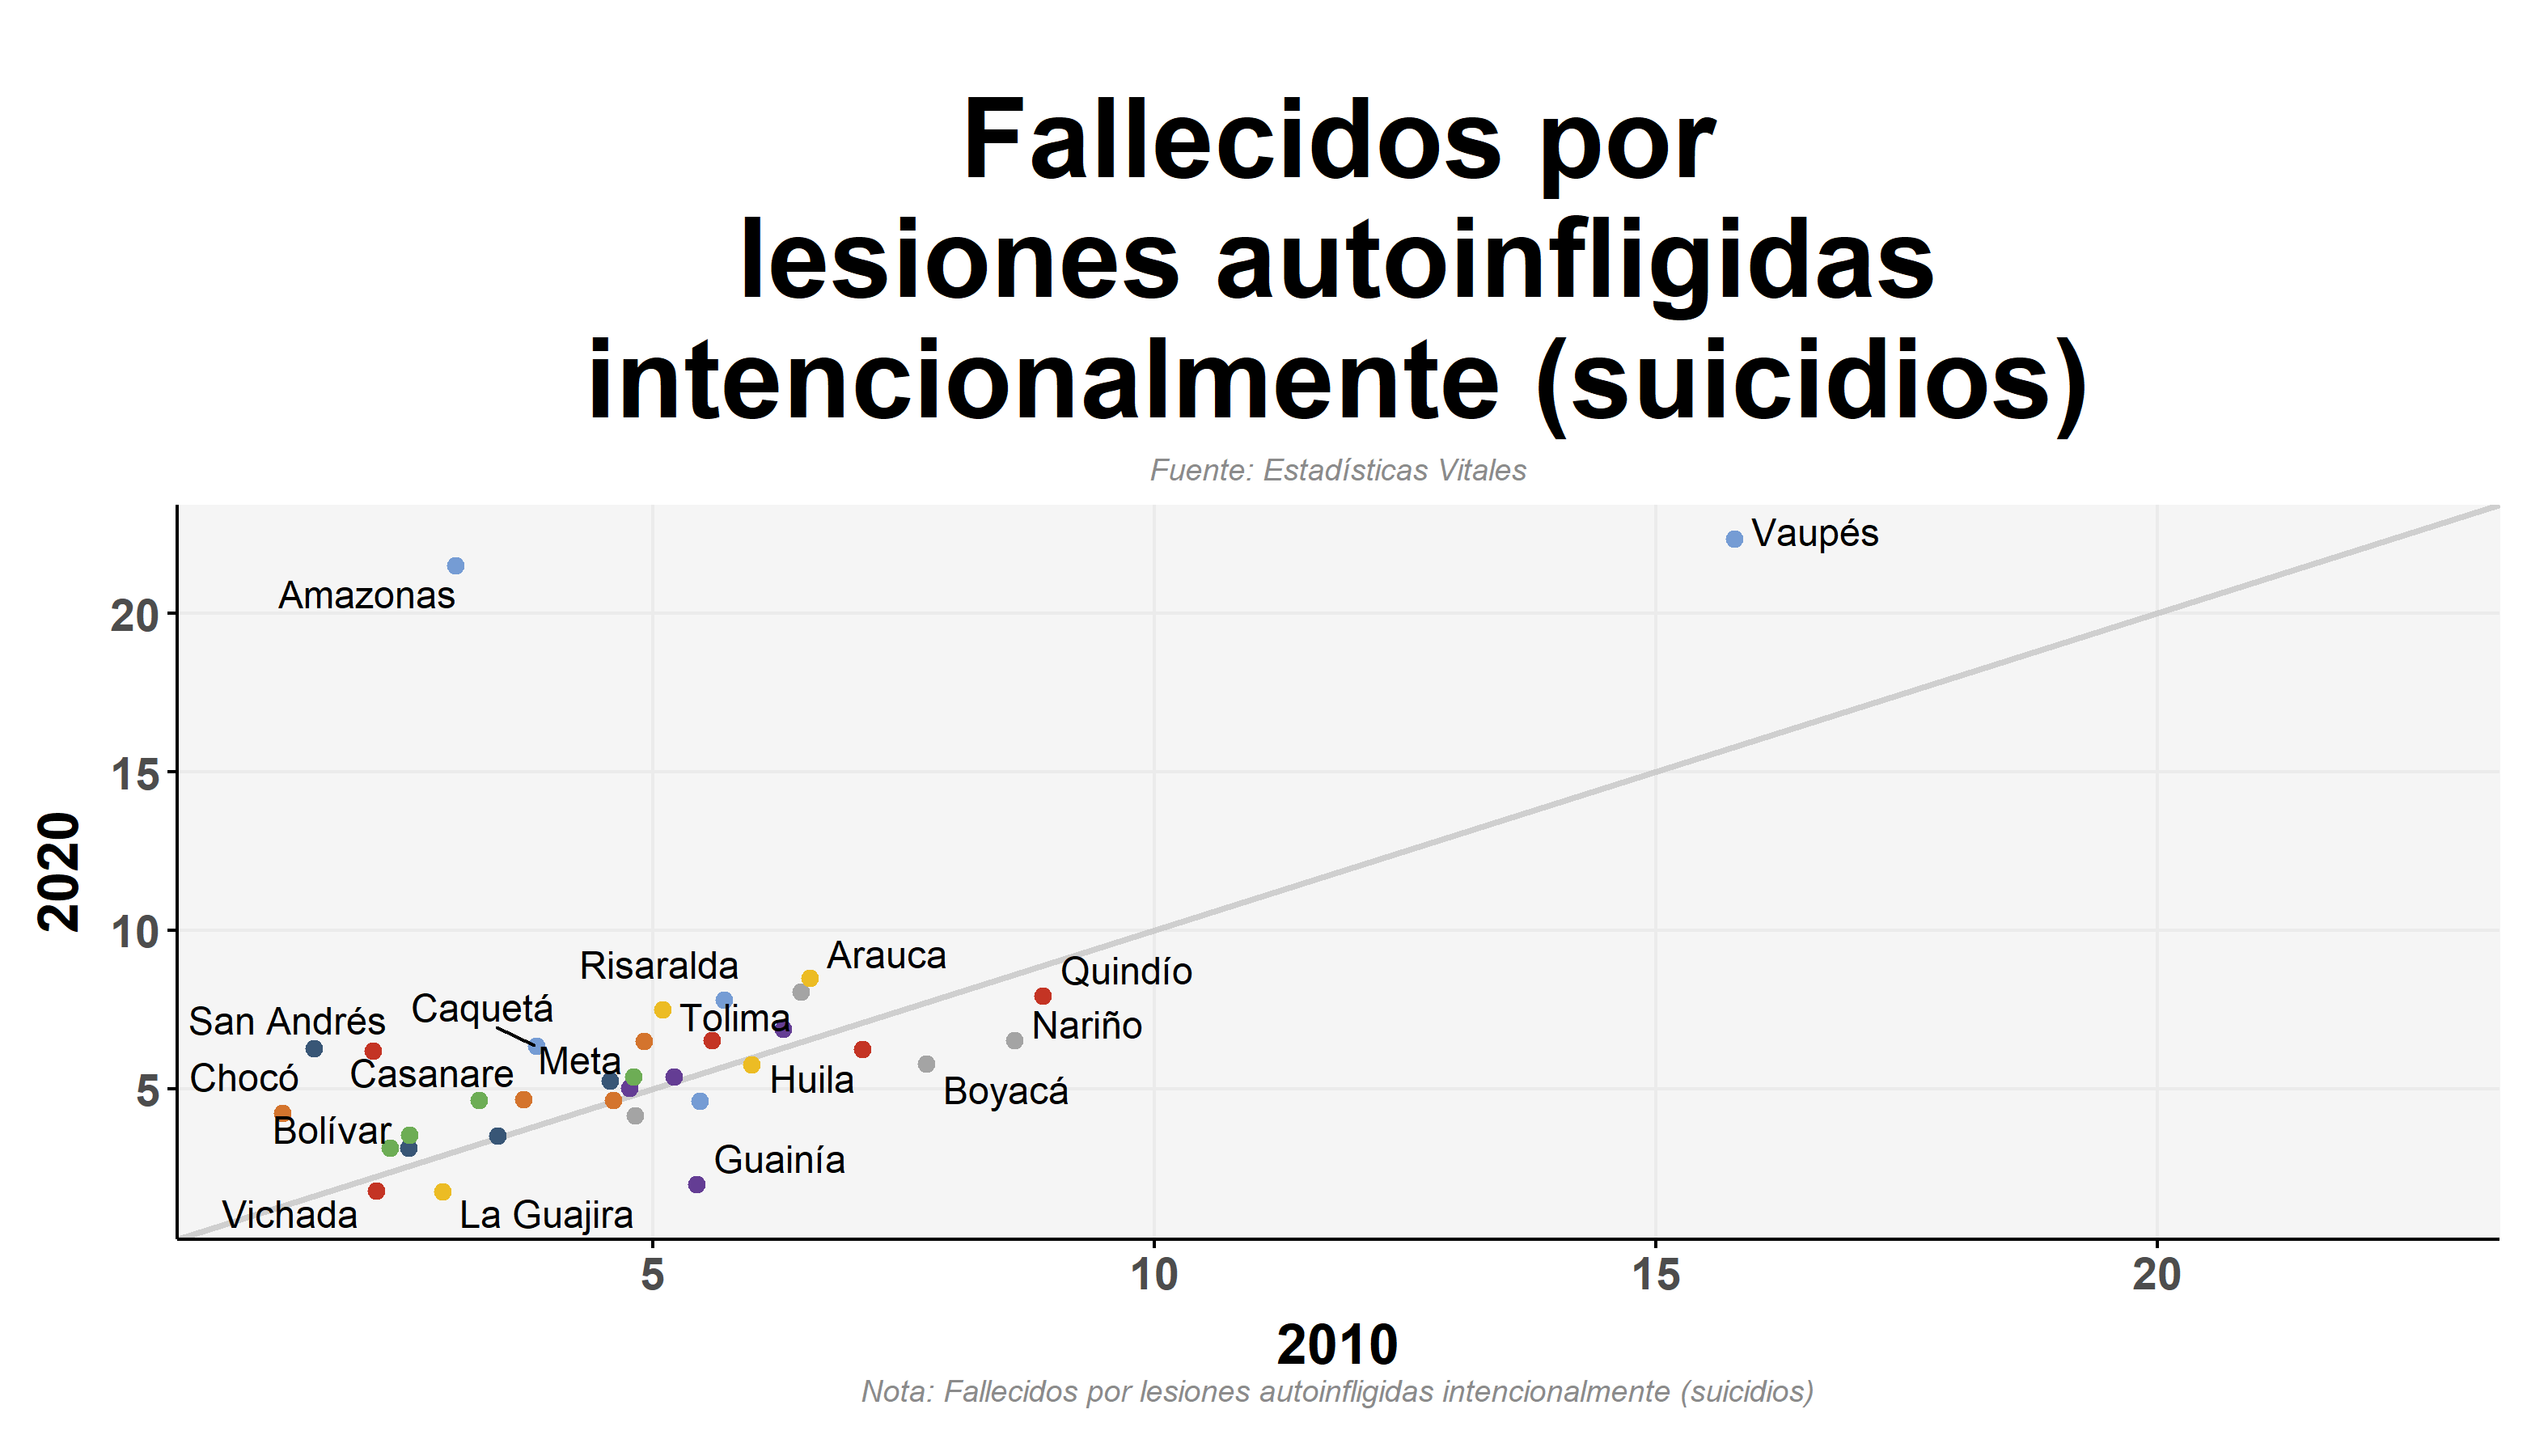
\includegraphics[width=\columnwidth]{img/var_324_scatter_time.png}
            \end{imagecolumn}
            \begin{textcolumn}
                \begin{itemize}
                    \item Hay una gran variación geográfica en la calidad de la educación primaria, medida como el tamaño de clase. 
                    \item Coexisten regiones con 25 estudiantes por docente (Atlántico) junto con regiones con tan sólo 12 estudiantes por docente (Guaviare)  
                    \item A pesar de que el tamaño de clase promedio nacional no cambió mucho entre 2014 y 2020, departamentos como Vichada y Amazonas experimentaron aumentos importantes en el tamaño de clase.
                \end{itemize}
            \end{textcolumn}

    \printcolumns
    \end{slide}
    
    
      %%% ----------------------------
    %%% Juventud
    %%% ----------------------------
    \subsection{Juventud}
    
    %%%-- Educación Superior
    \begin{slide}{14} 
                      \begin{imagecolumn}
                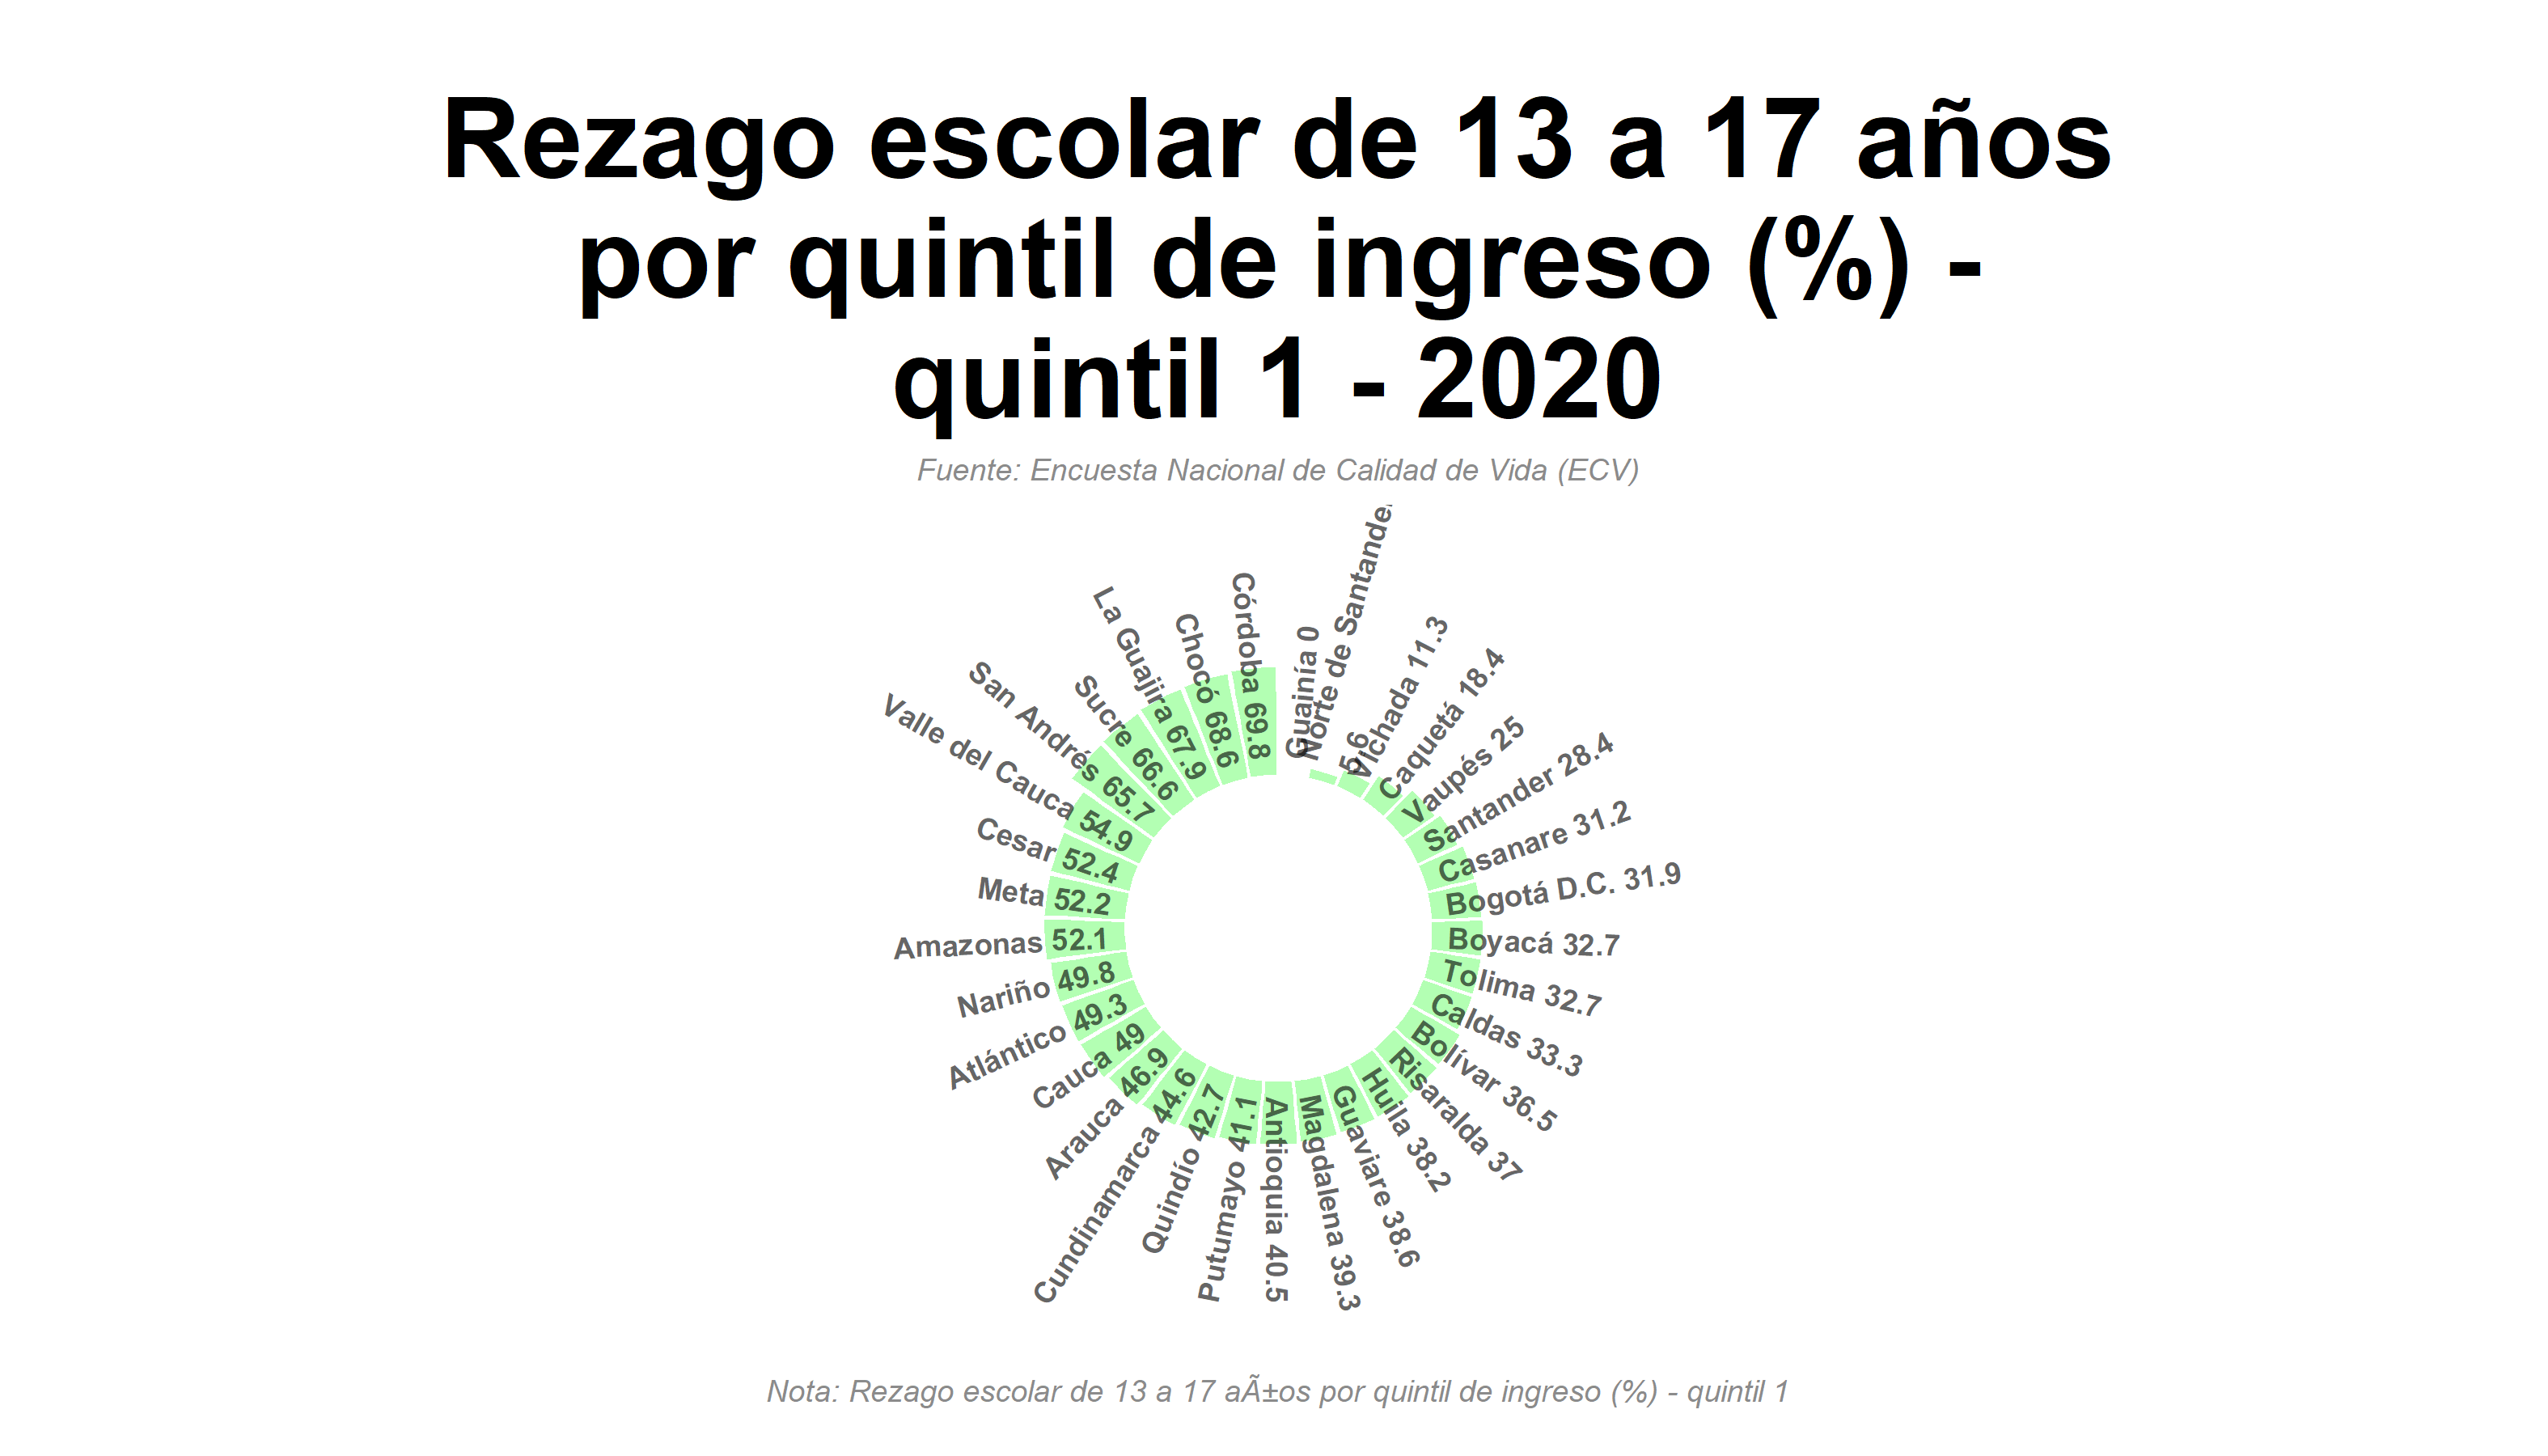
\includegraphics[width=\columnwidth]{img/var_211_static.png}
            \end{imagecolumn}
            \begin{textcolumn}
                \begin{itemize}
                    \item Existe una alta desigualdad en el acceso a la educación superior entre regiones
                    \item Mientras que en Bogotá el 43% de los jóvenes ha asistido a institutos de educación superior por al menos 1 año, en Vichada éste porcentaje es de sólo 7%
                    \item Éstas diferencias no han cambiado mucho en el tiempo 
                \end{itemize}
            \end{textcolumn}

    \printcolumns
    \end{slide}
    
    %%%-- Fertilidad 
    \begin{slide}{14} 
            \begin{imagecolumn}
                \includegraphics[width=\columnwidth]{img/var_297_map.png}
            \end{imagecolumn}
            \begin{textcolumn}
                \begin{itemize}
                    \item Progresivamente, Colombia se va convirtiendo en un país menos fértil
                    \item Aunque regiones como Chocó, Guajira y Amazonas siguen teniendo altas tasas de fertilidad
                \end{itemize}
            \end{textcolumn}

    \printcolumns
    \end{slide}
    
        %%%-- NINIS 
    \begin{slide}{14} 
                      \begin{imagecolumn}
                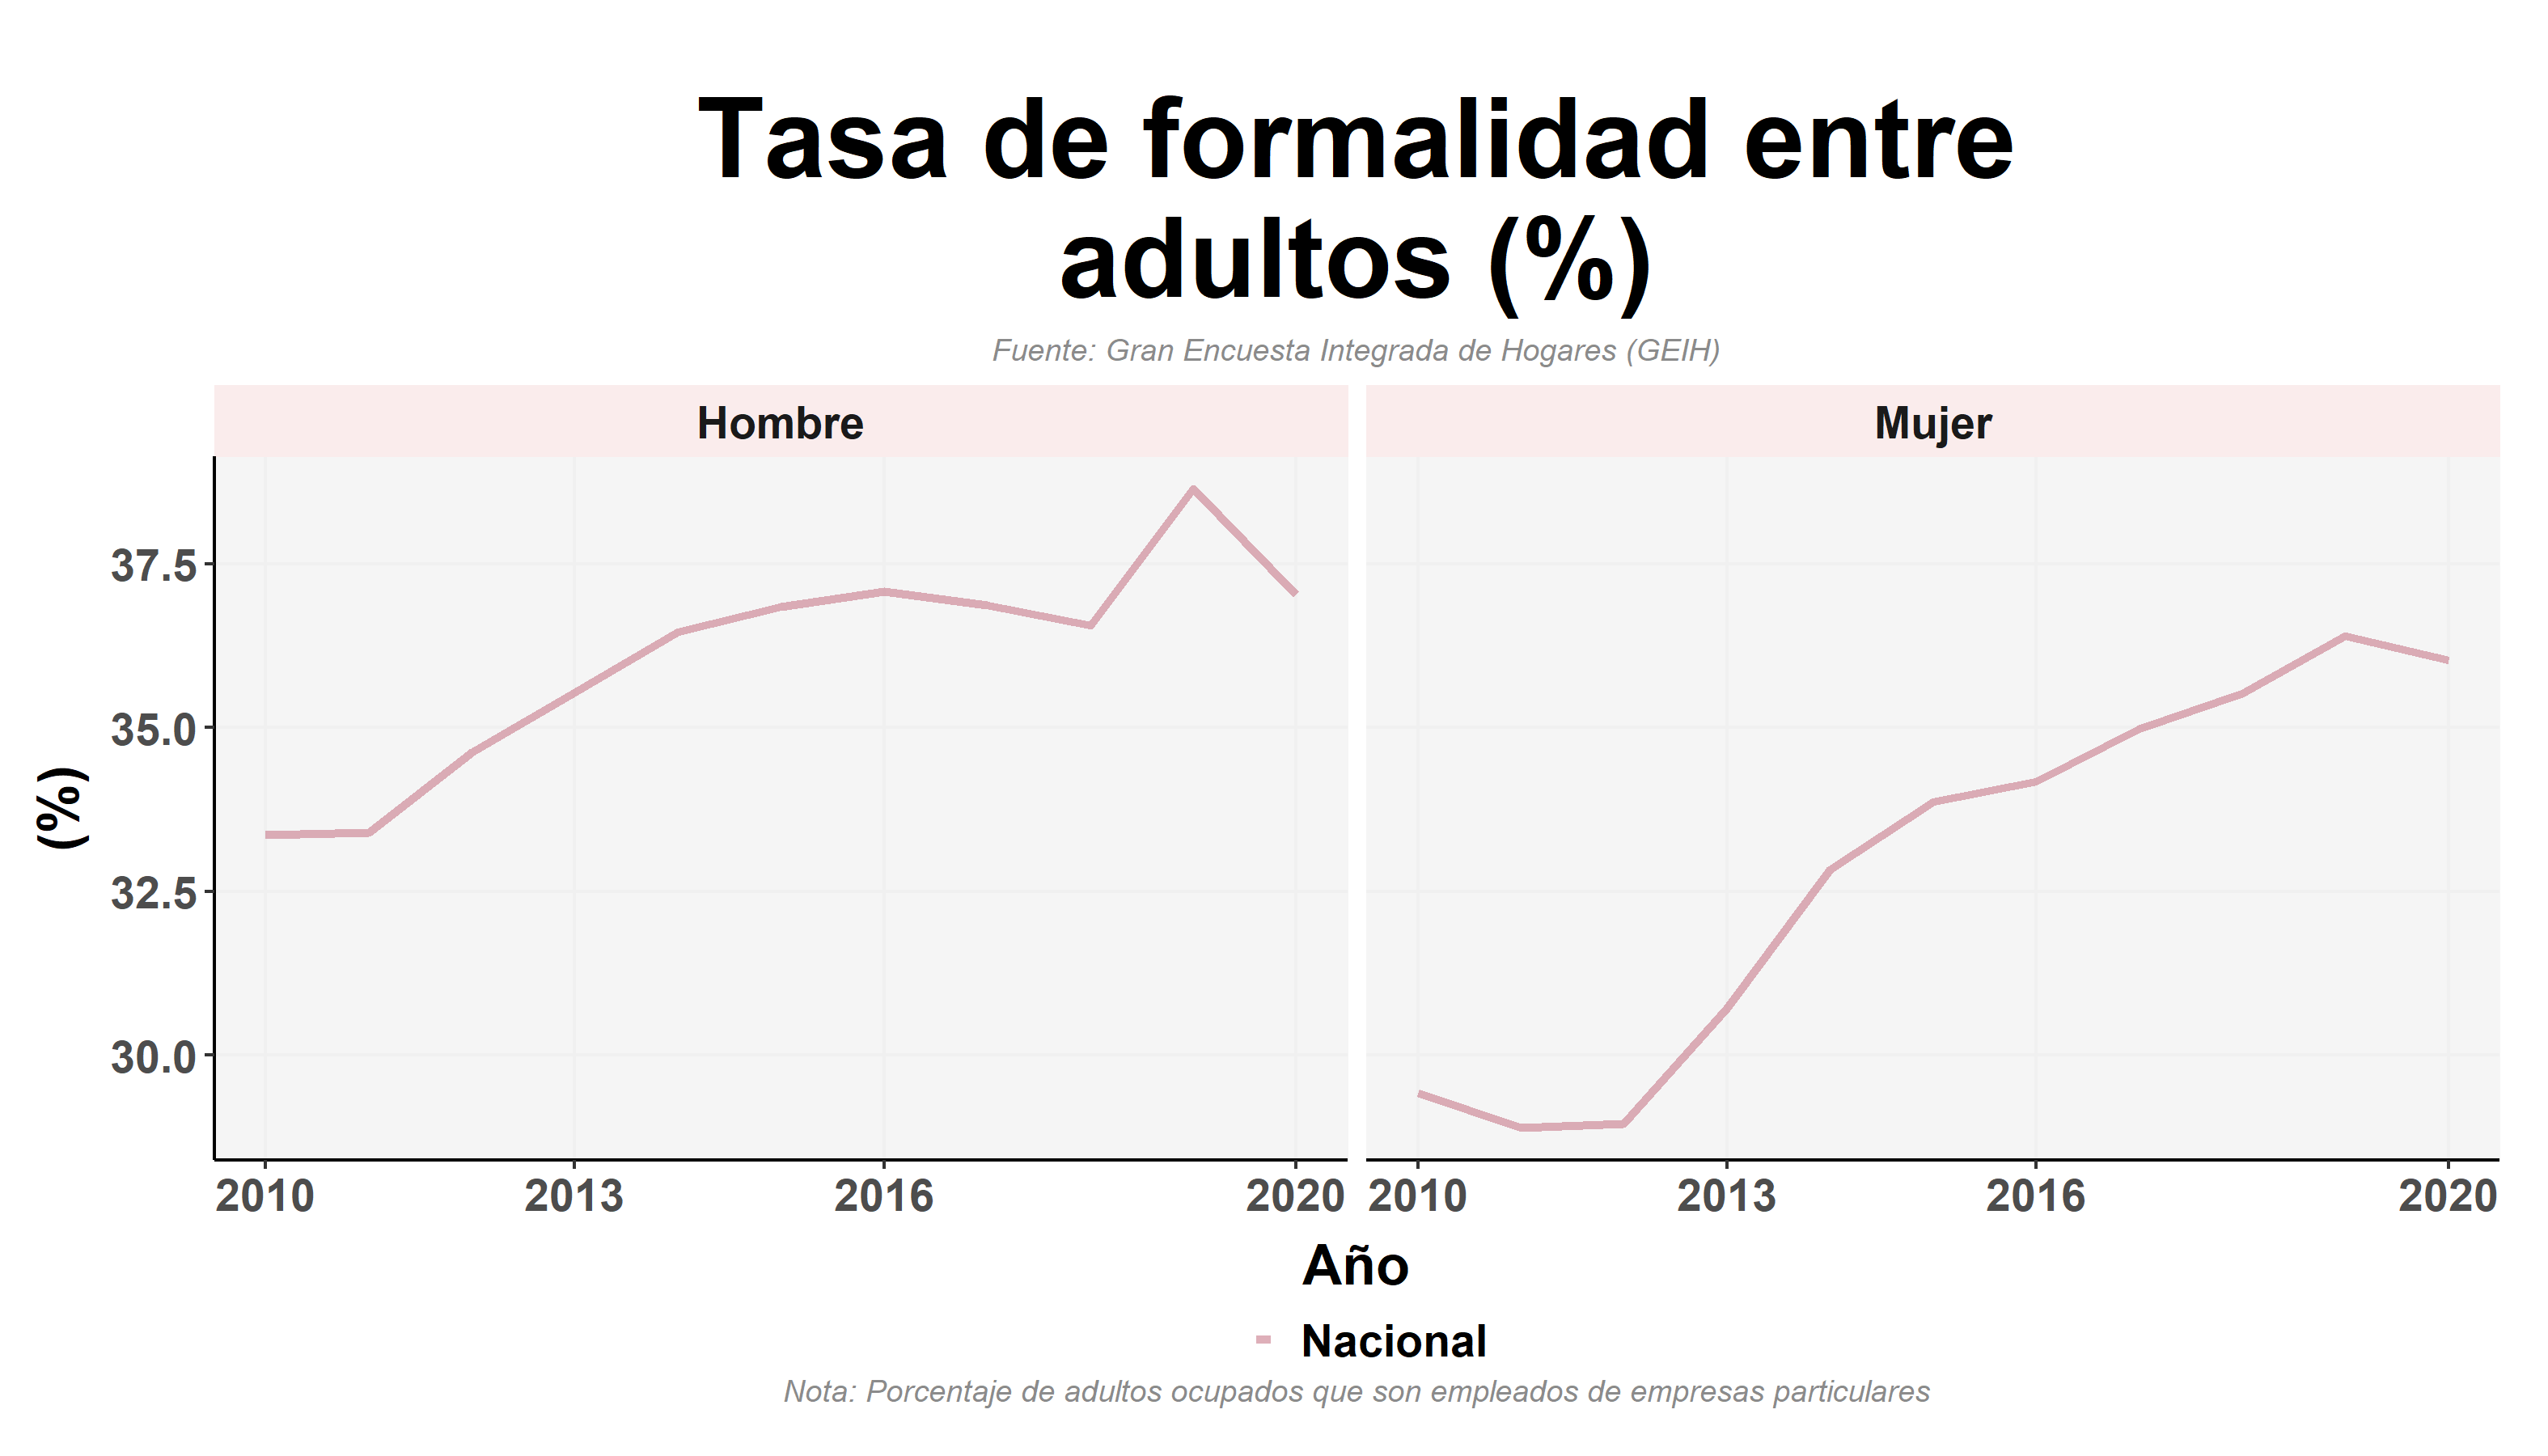
\includegraphics[width=\columnwidth]{img/var_81_trend.png}
            \end{imagecolumn}
            \begin{textcolumn}
                \begin{itemize}
                    \item La tasa de mujeres jóvenes que ni estudian, ni trabajan es casi el doble que la de los hombres jóvenes
                    \item Esta tendencia se agudizó con la pandemia.
                \end{itemize}
            \end{textcolumn}

    \printcolumns
    \end{slide}
    
    %%%-- Desempleo 
    \begin{slide}{14} 
            \begin{imagecolumn}
                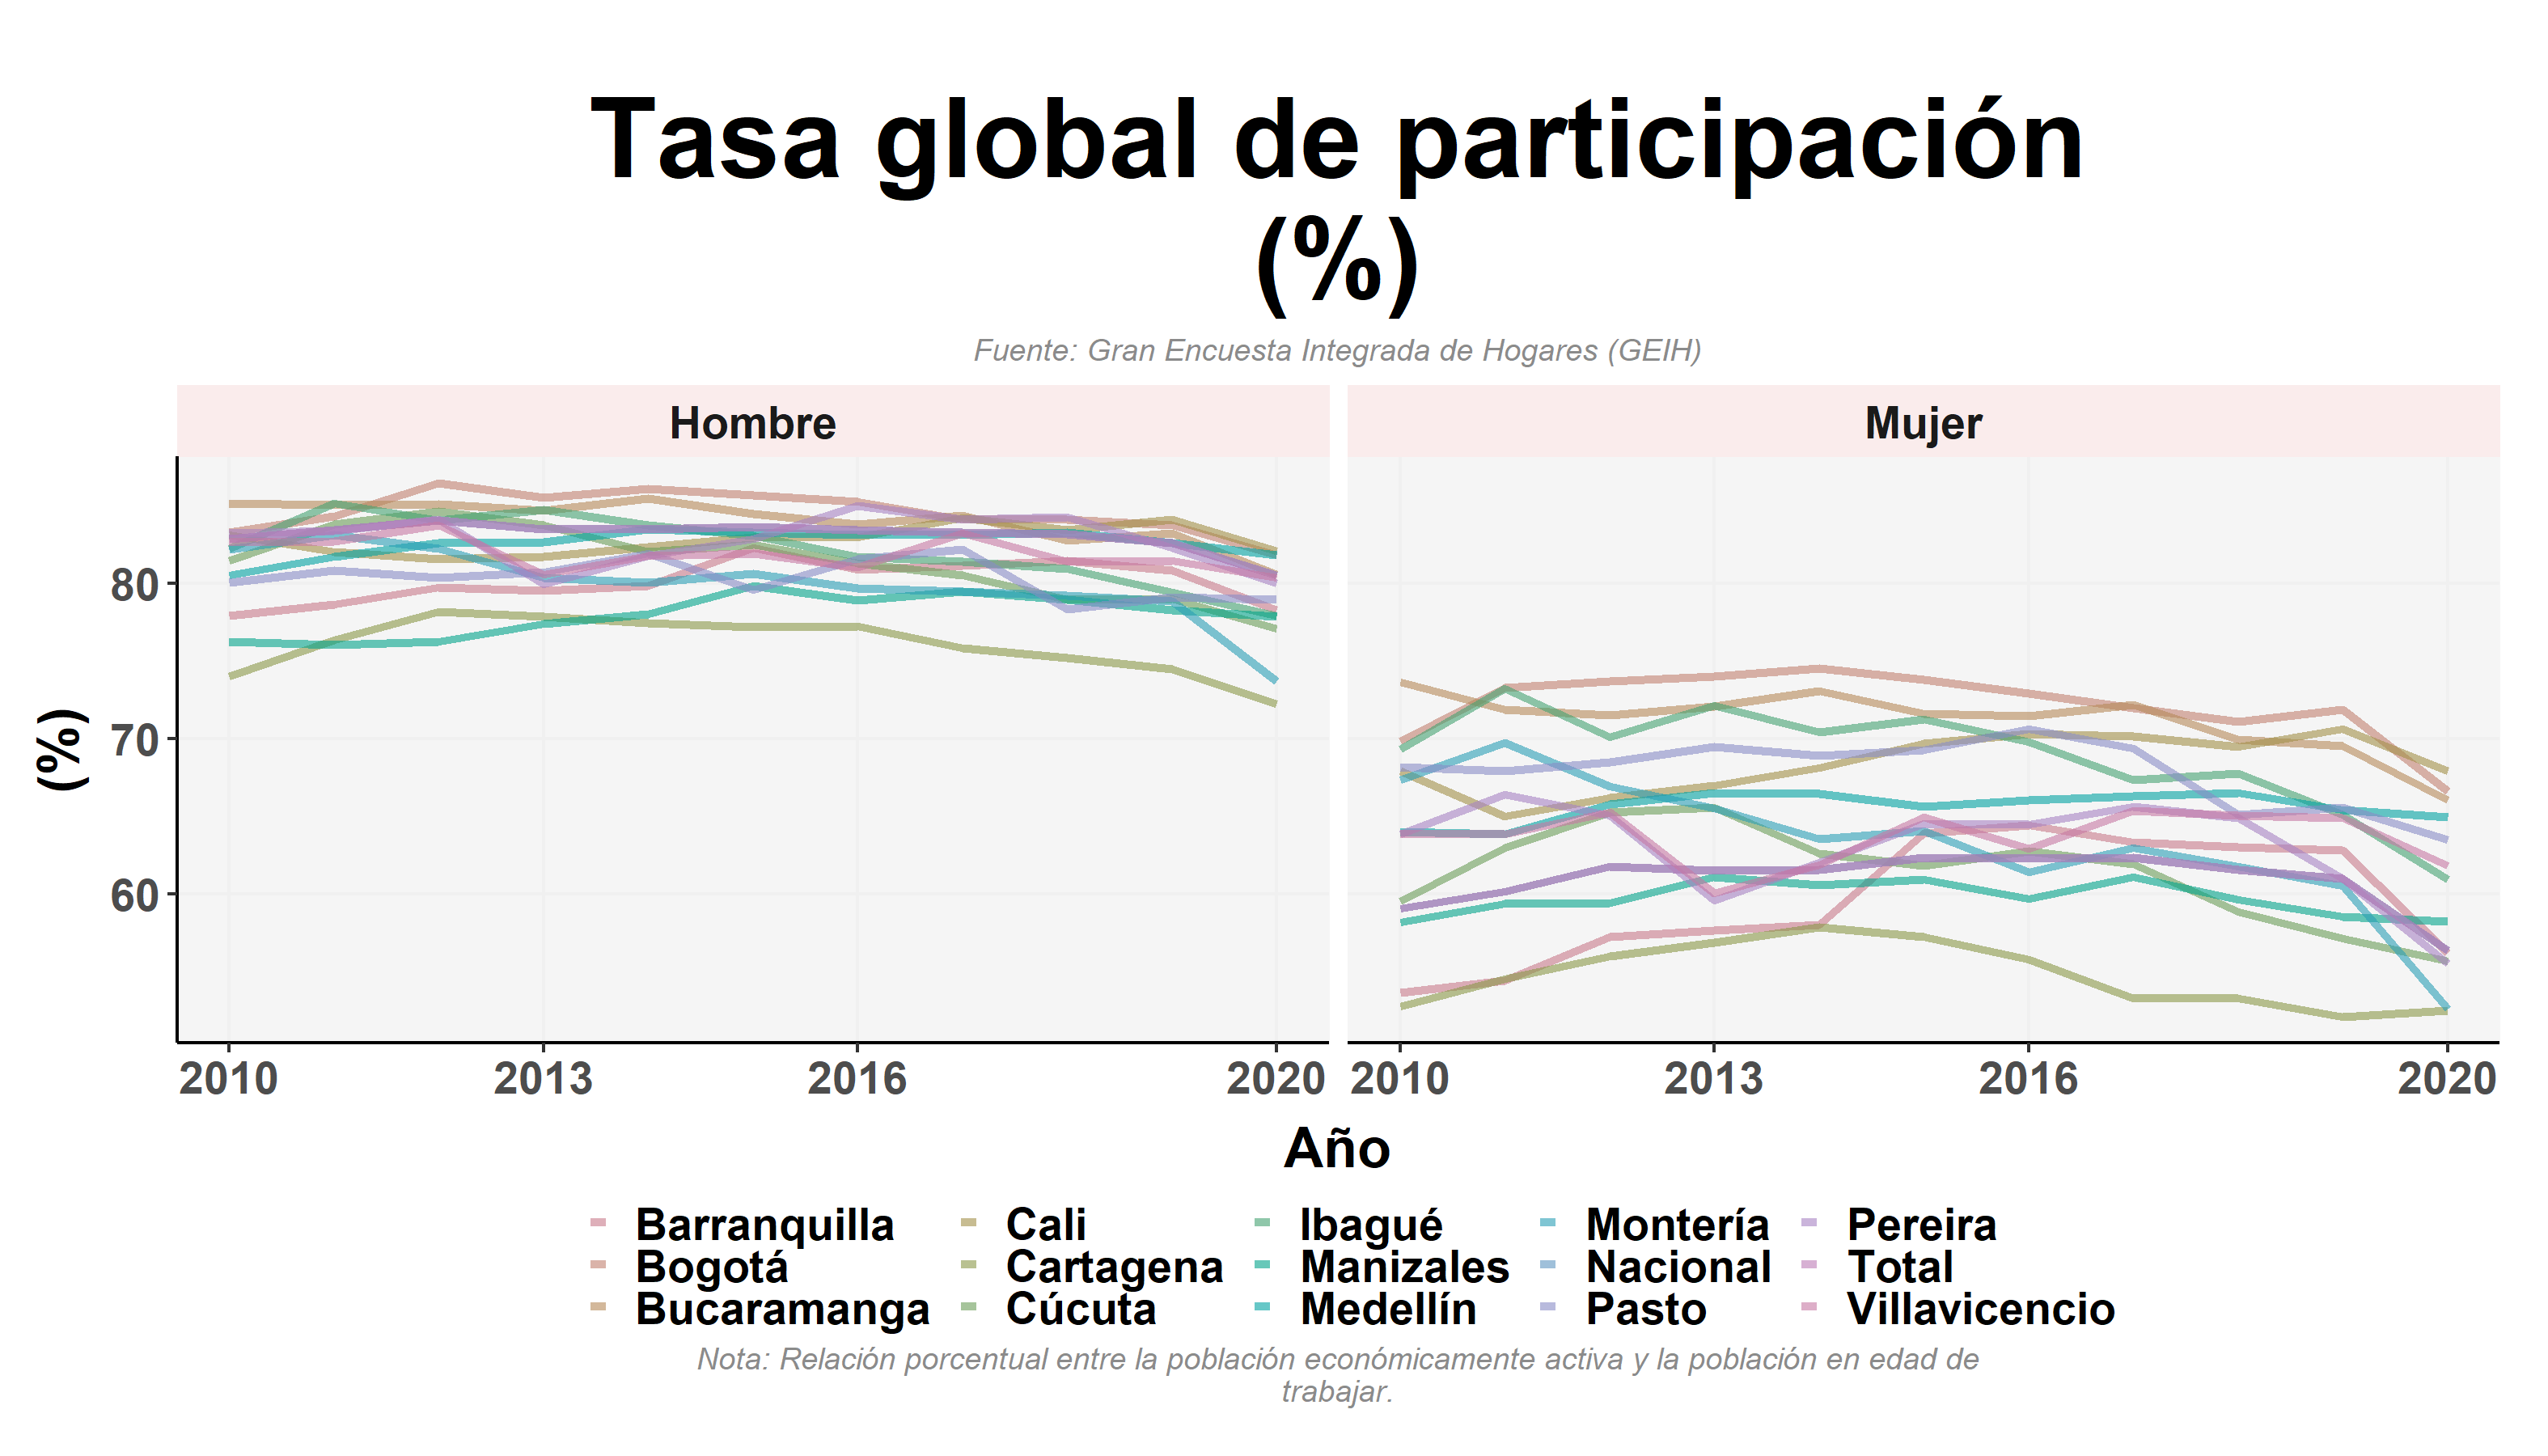
\includegraphics[width=\columnwidth]{img/var_102_trend.png}
            \end{imagecolumn}
            \begin{textcolumn}
                \begin{itemize}
                    \item La diferencia en la tasa de desempleo entre hombre y mujer, 
                    \item Esta tendencias se agudizó con la pandemia
                \end{itemize}
            \end{textcolumn}
    \printcolumns
    \end{slide}
    
        %%%-- Highlights 
    \begin{slide}{14} 
            \begin{imagecolumn}
                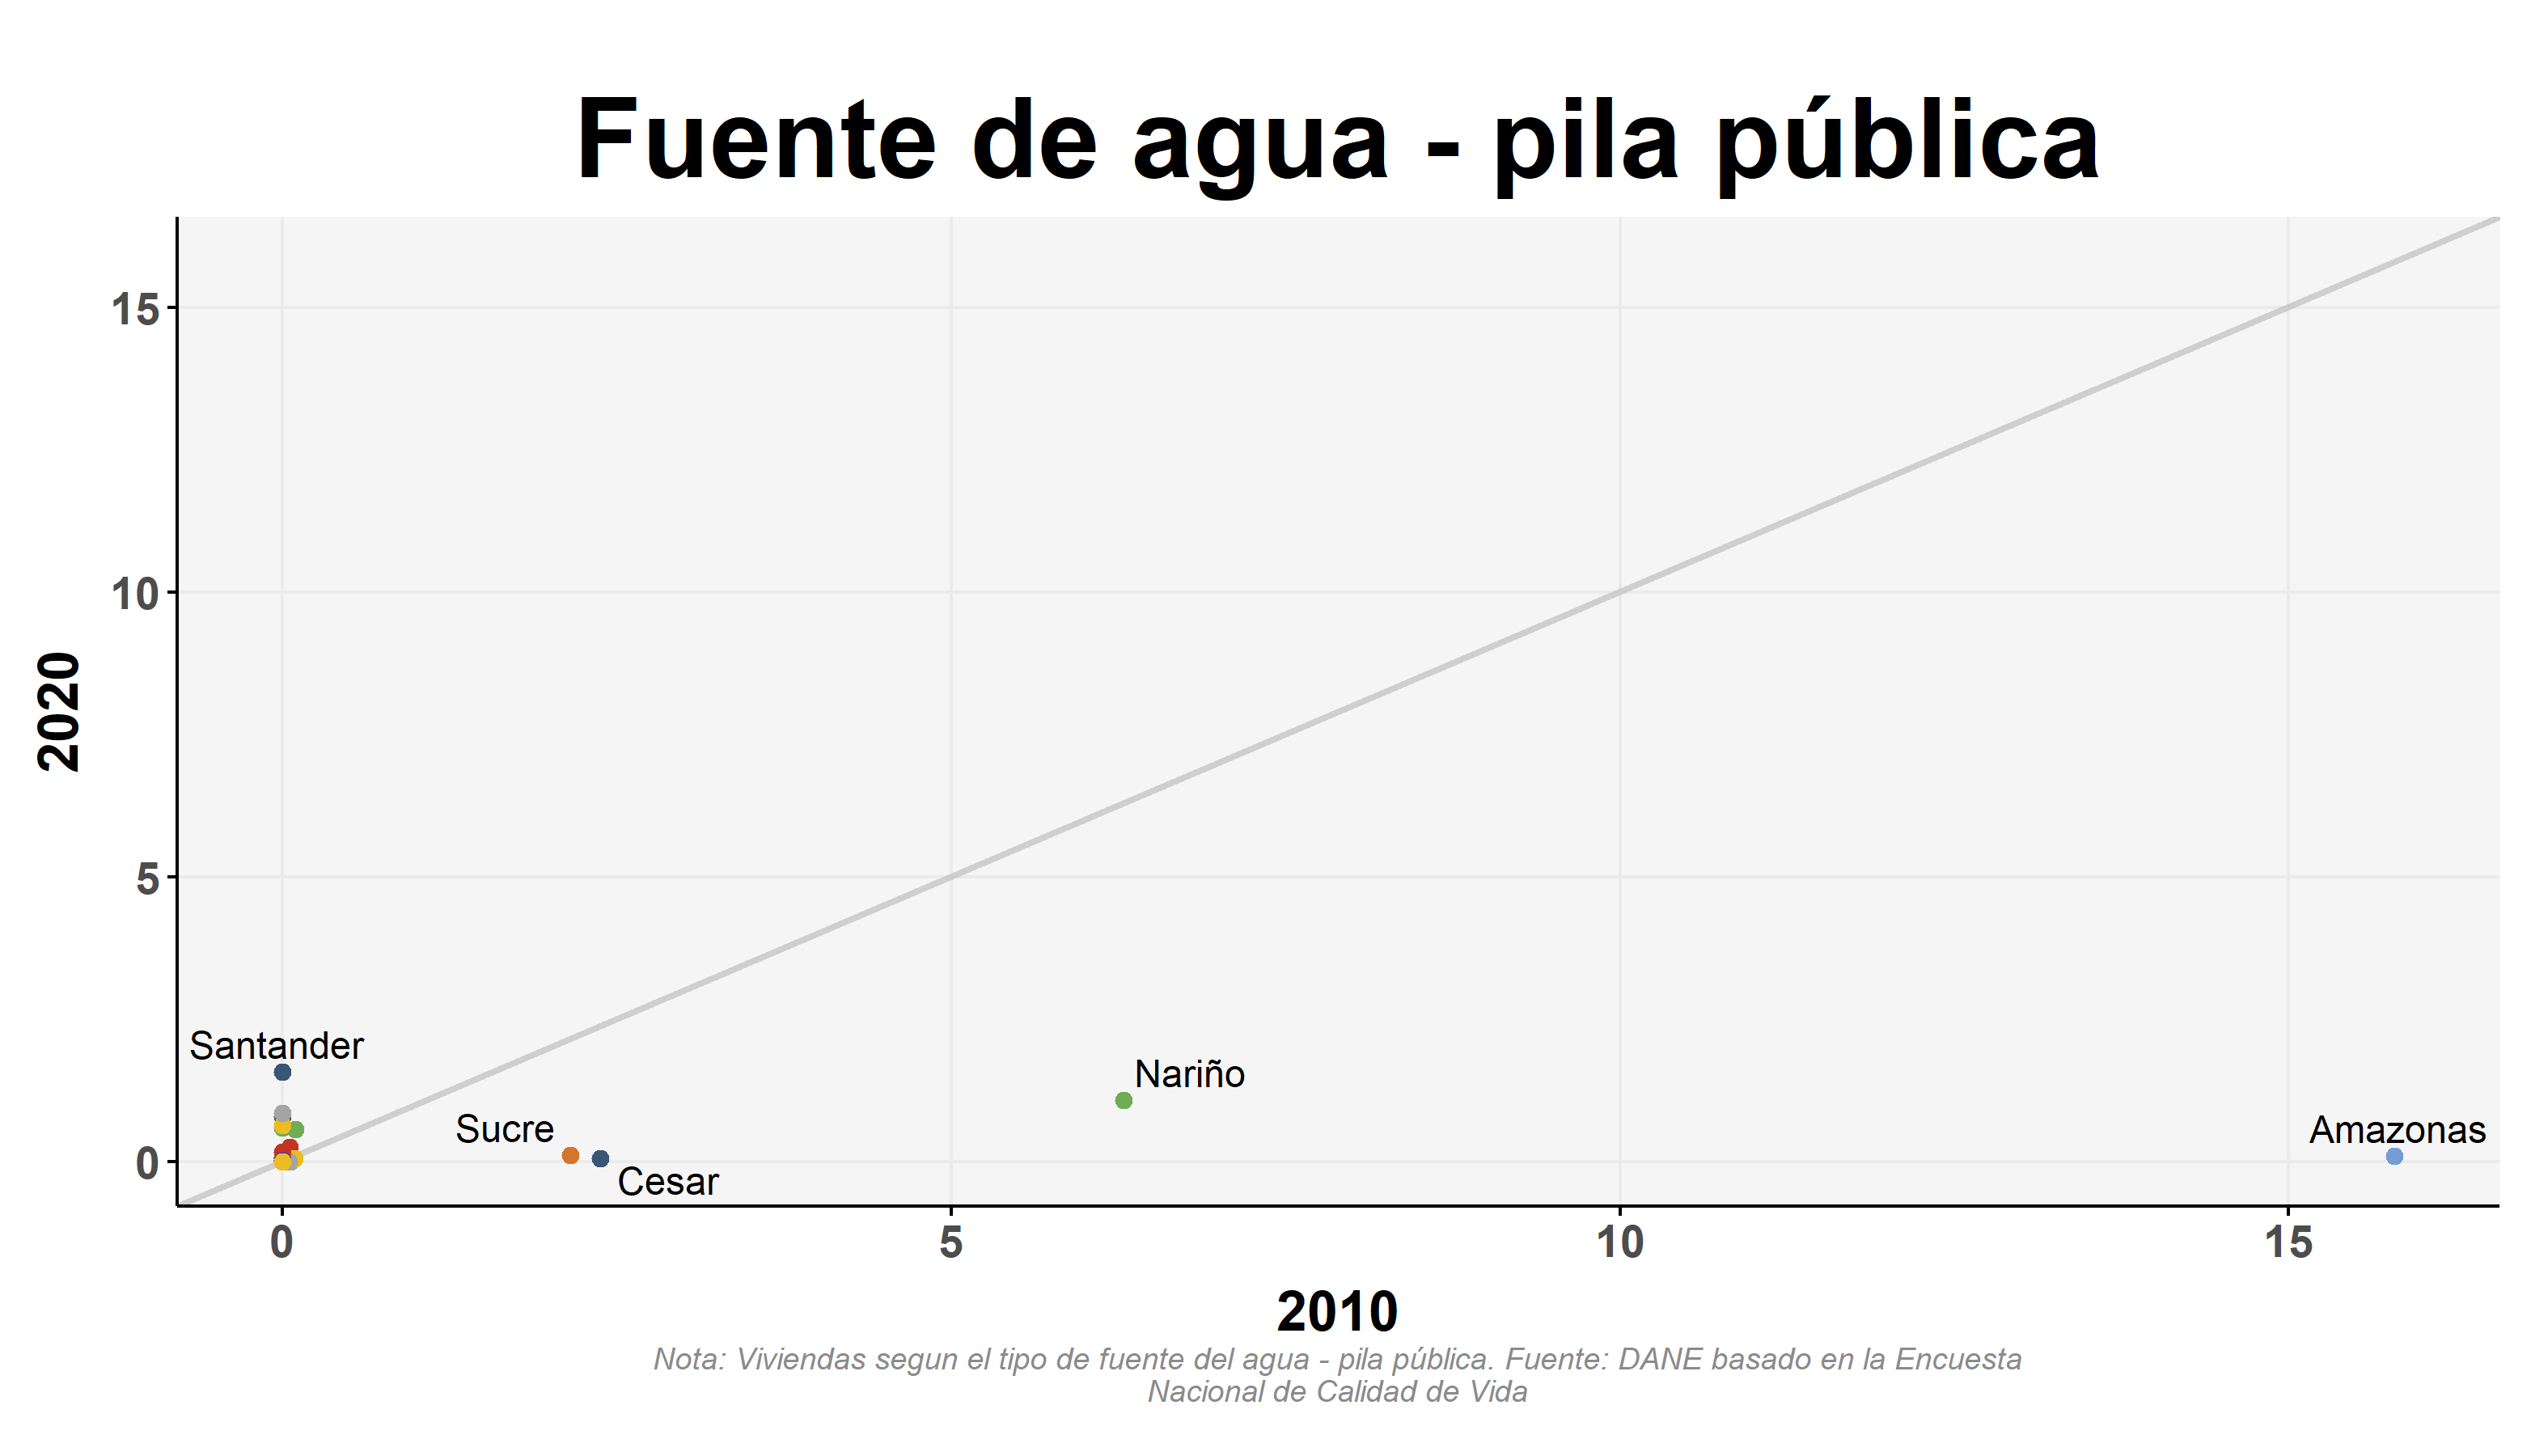
\includegraphics[width=\columnwidth]{img/var_145_scatter_time.png}
            \end{imagecolumn}
            \begin{textcolumn}
                \begin{itemize}
                    \item Las tendencias de la informalidad se ha mantenido constante, aunque en algunas regiones se ha agudizado 
                \end{itemize}
            \end{textcolumn}
    \printcolumns
    \end{slide}
    
      %%% ----------------------------
    %%% Cambio Climático
    %%% ----------------------------
    \subsection{Adultez}
    
            %%%-- Highlights 
    \begin{slide}{15} 
            \begin{imagecolumn}
                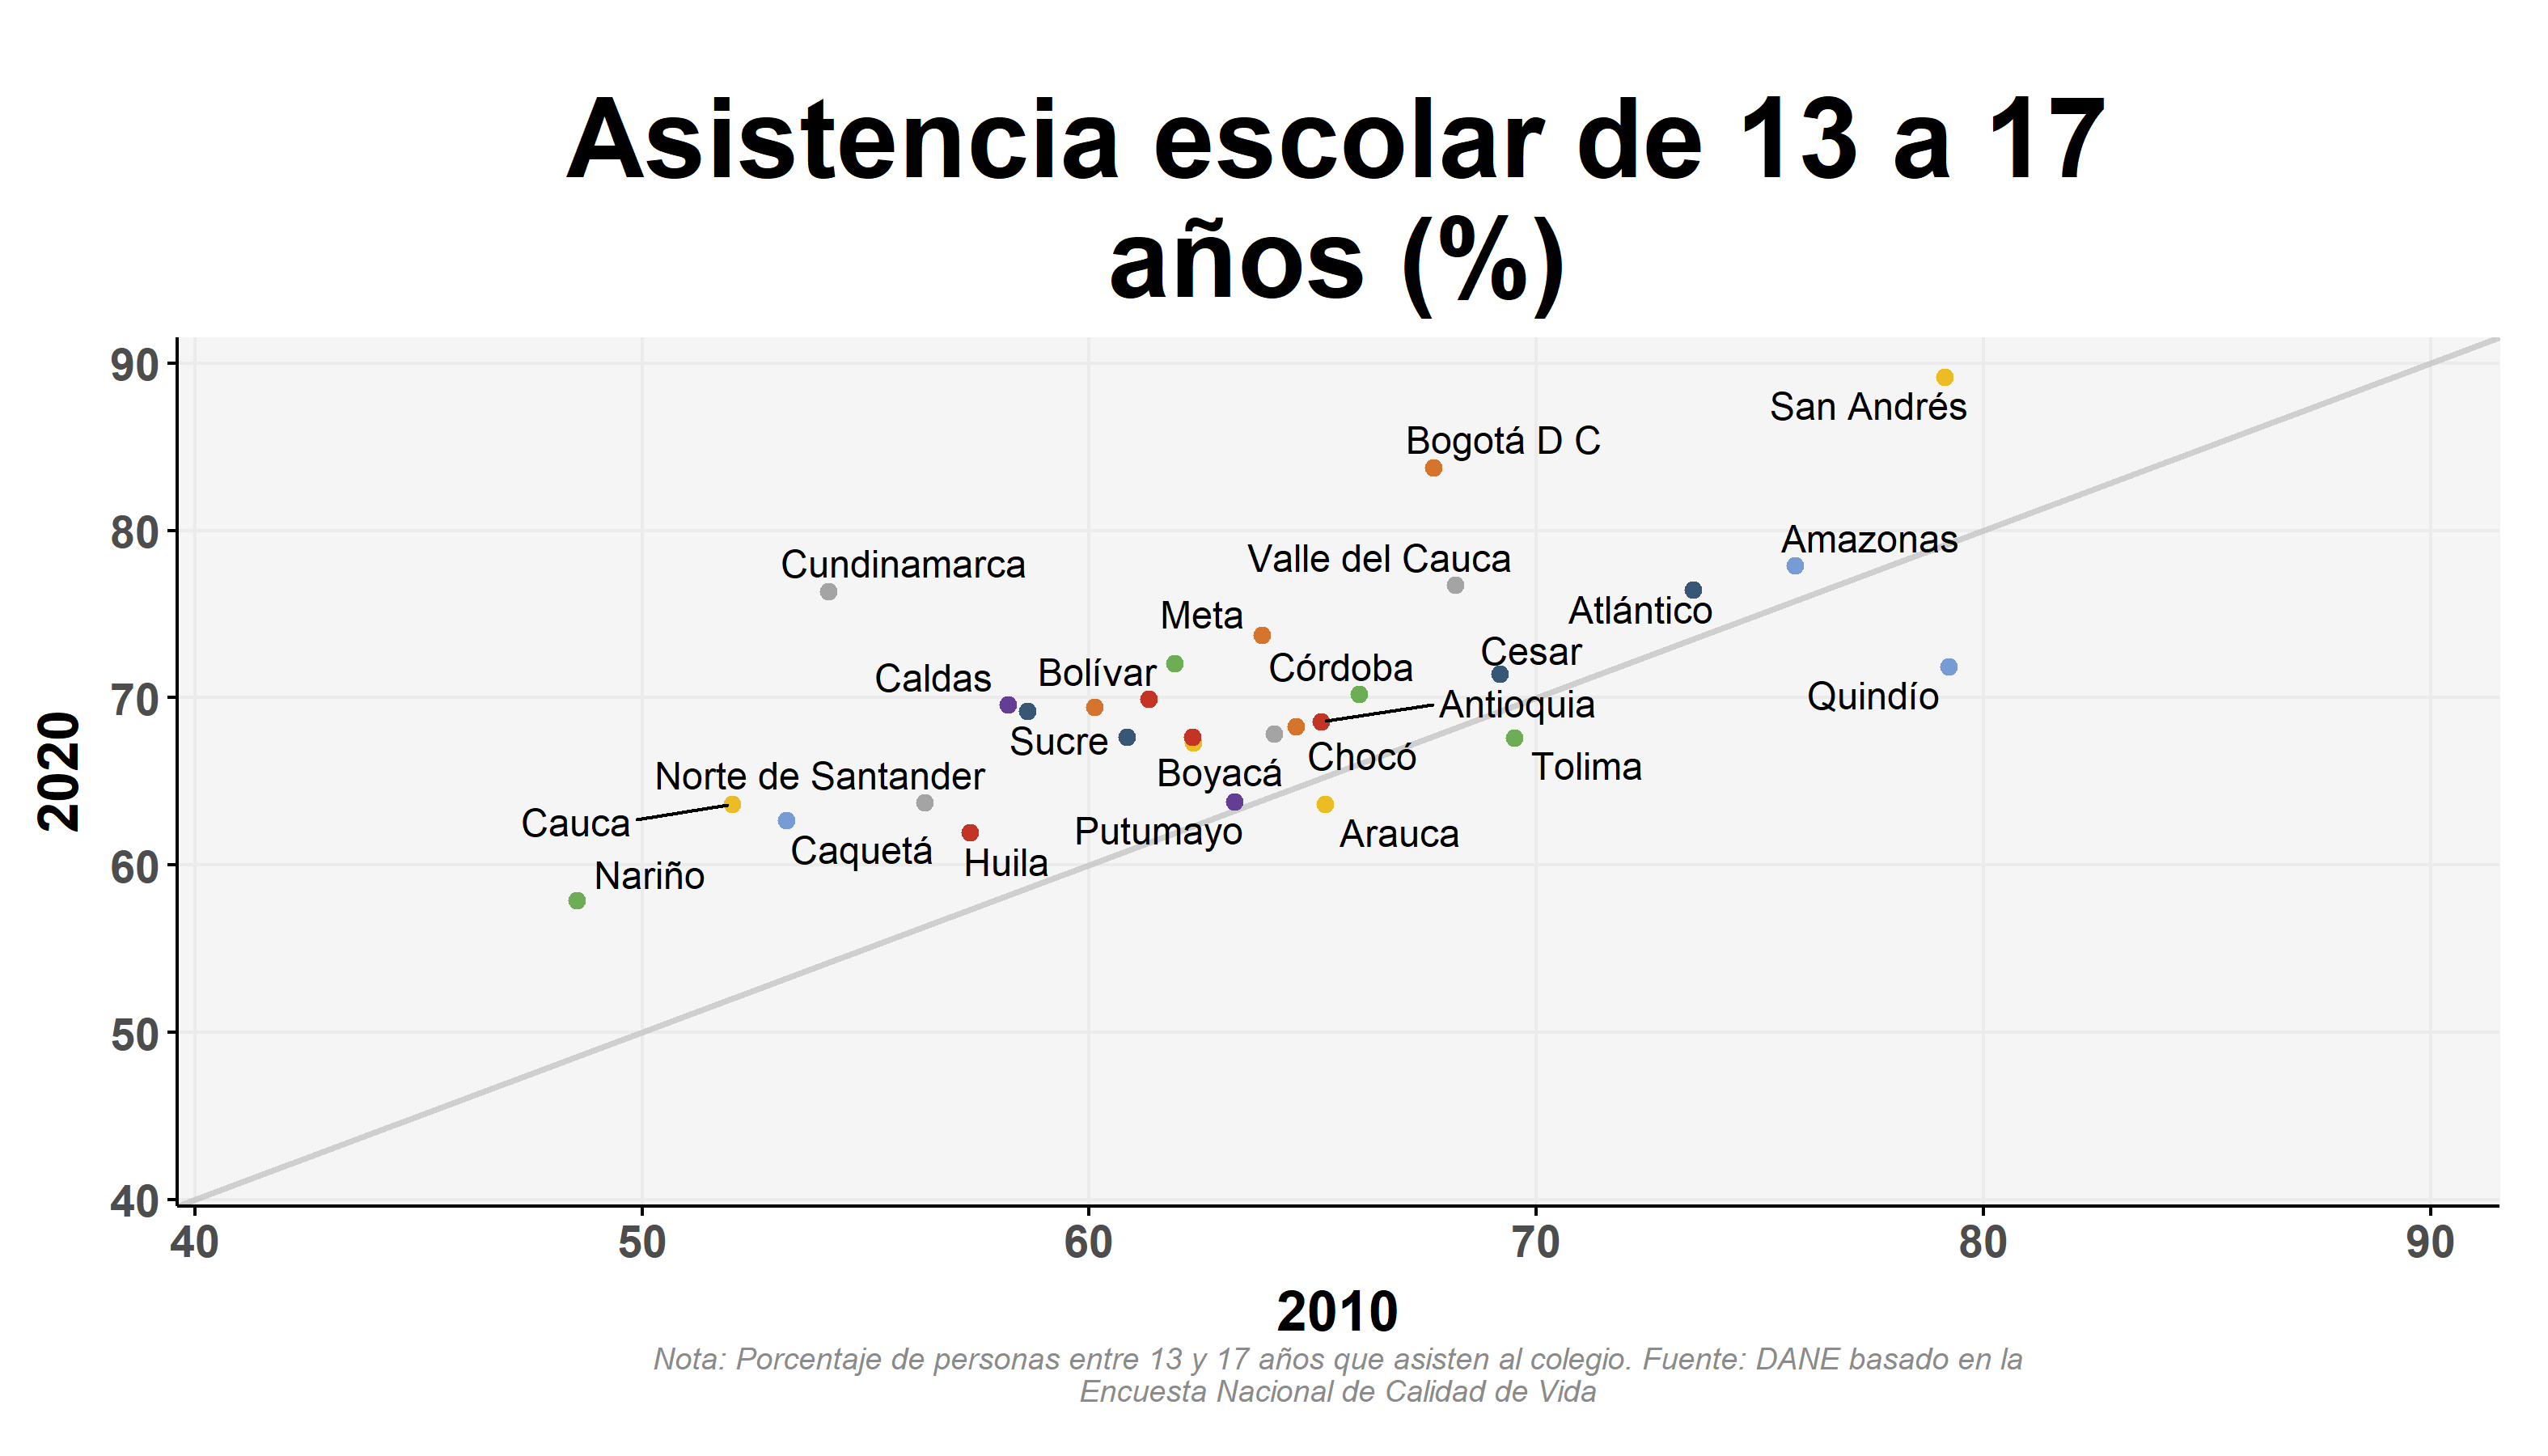
\includegraphics[width=\columnwidth]{img/var_87_scatter_time.png}
            \end{imagecolumn}
            \begin{textcolumn}
                \begin{itemize}
                    \item Un incremento en el desempleo generalizado debido a la pandemia
                    \item Con algunas ciudades donde se ha agudizado en mayor magnitud
                \end{itemize}
            \end{textcolumn}
    \printcolumns
    \end{slide}
    
    
        \begin{slide}{15} 
            \begin{imagecolumn}
                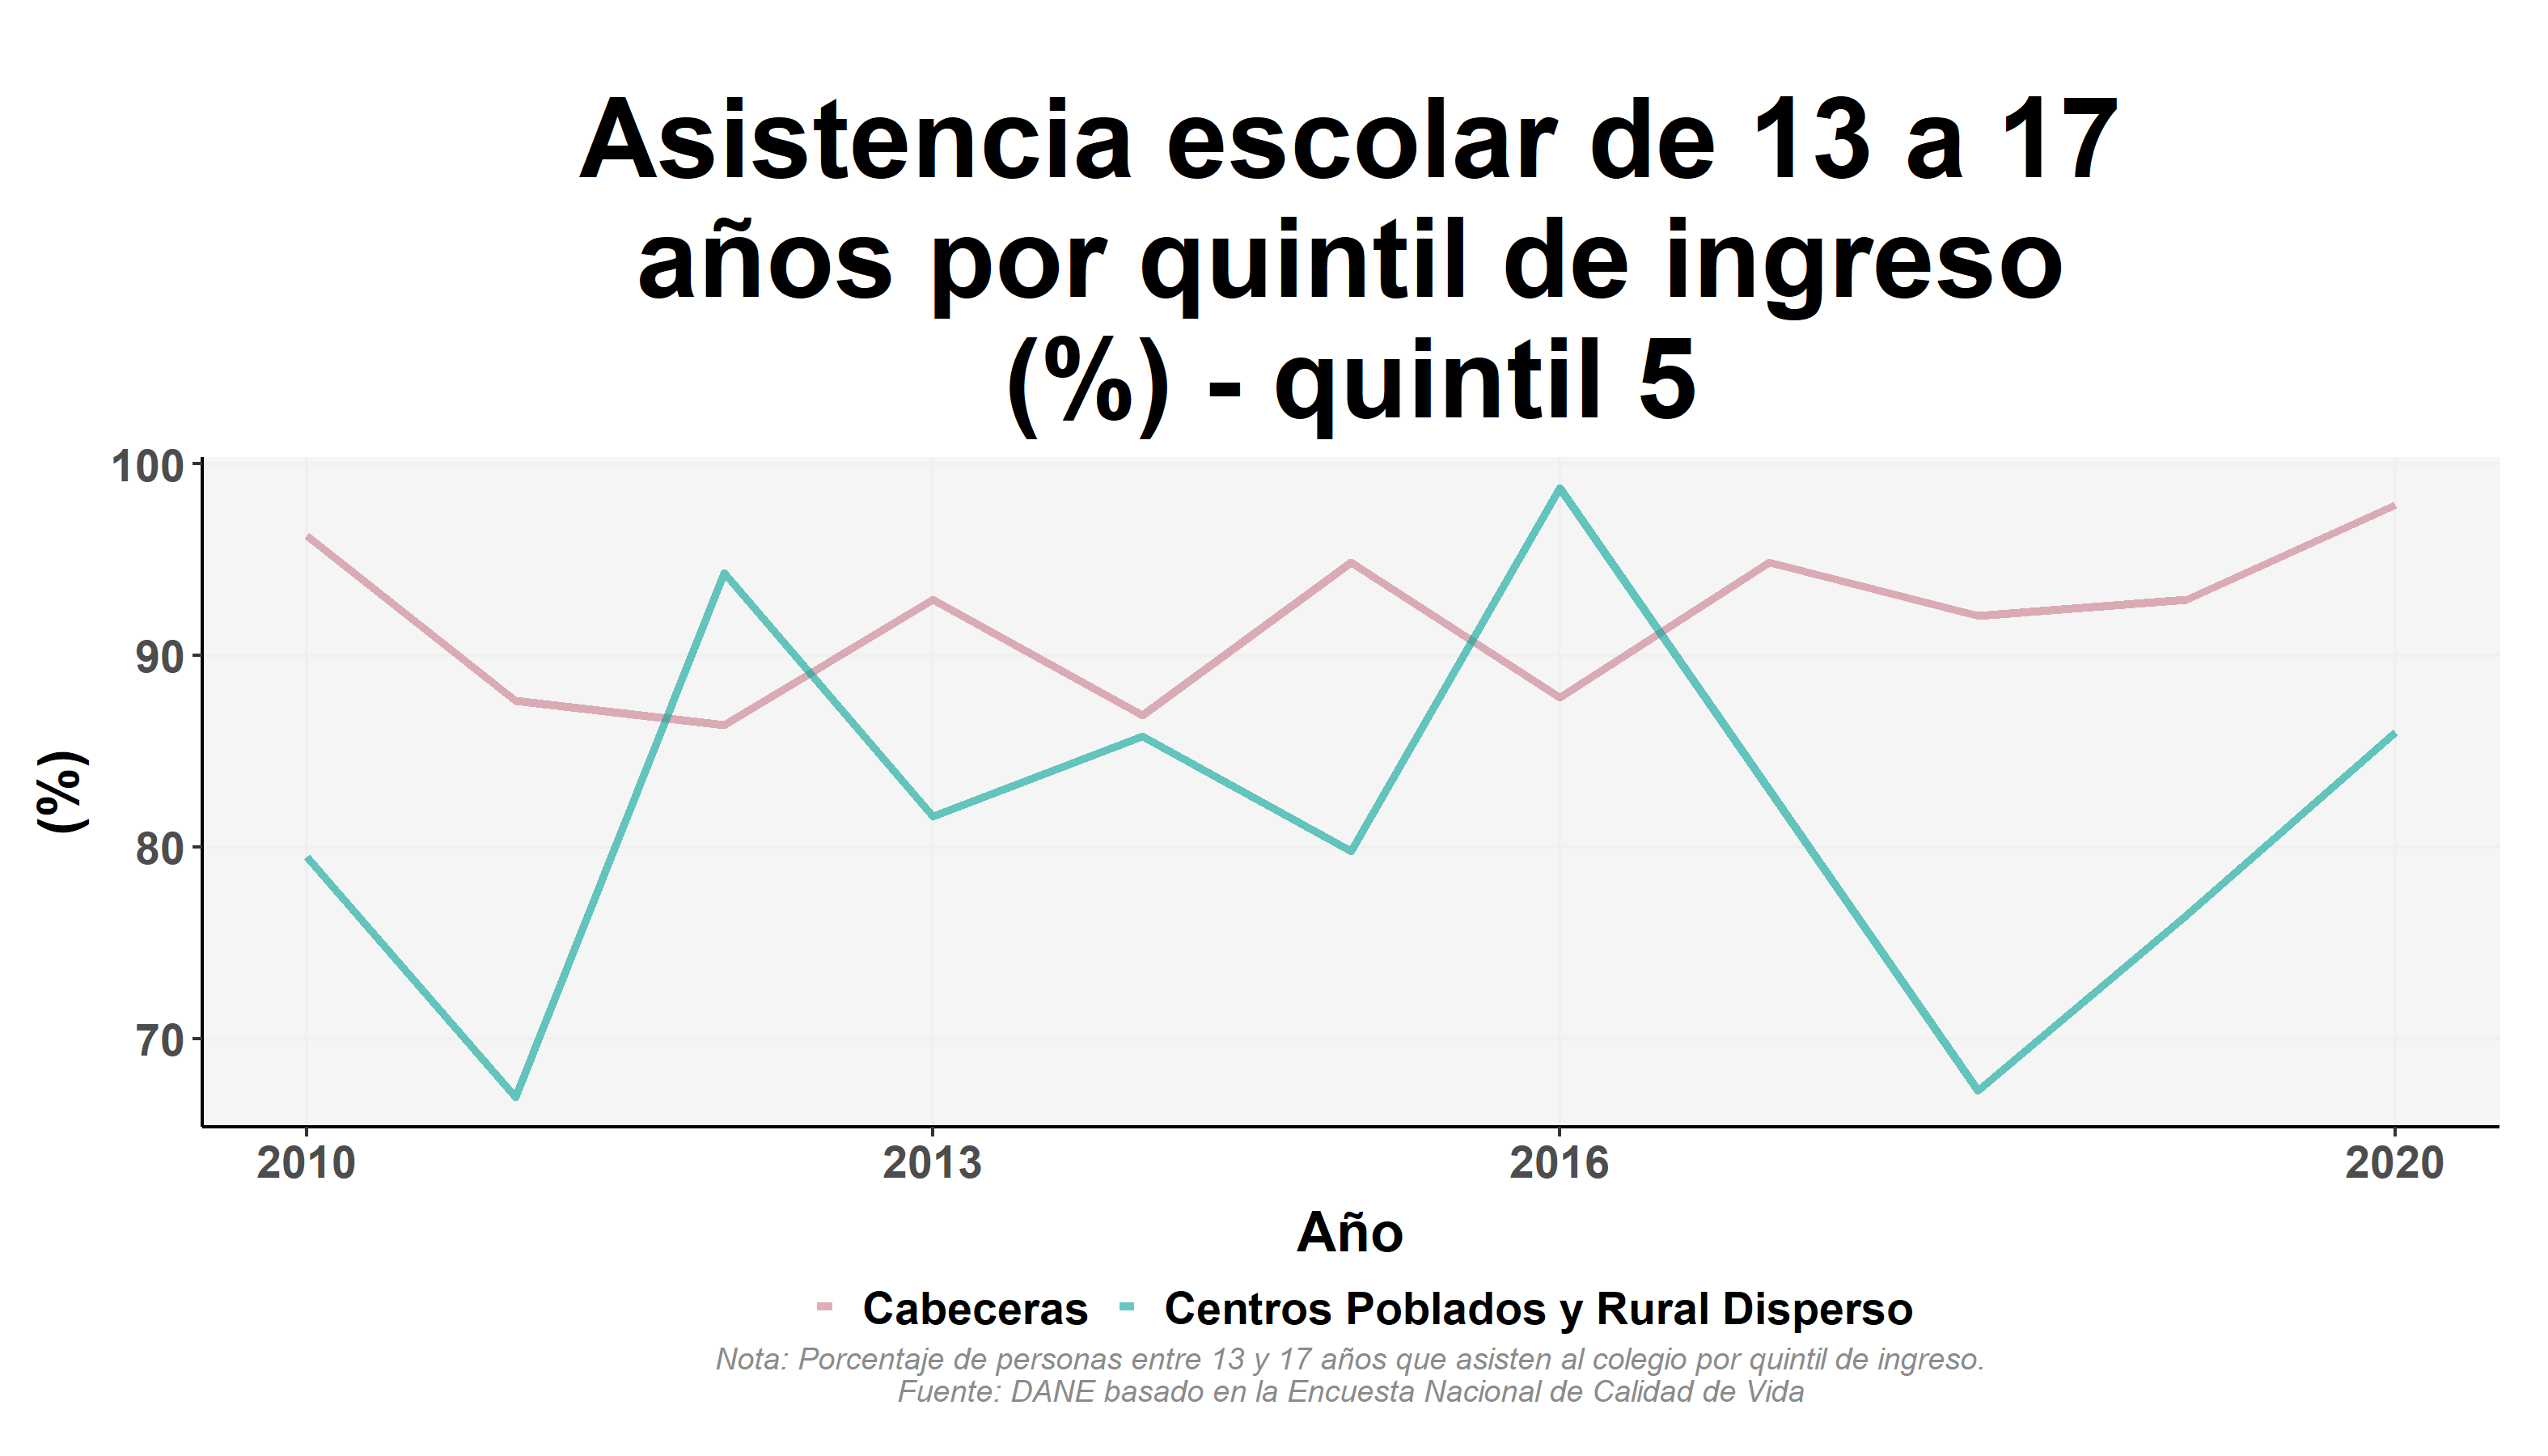
\includegraphics[width=\columnwidth]{img/var_98_trend.png}
            \end{imagecolumn}
            \begin{textcolumn}
                \begin{itemize}
                    \item Un incremento en el desempleo generalizado debido a la pandemia
                    \item La pandemia llevó a los hombres a tener las tasas de desempleo que las mujeres tenían hace diez años. 
                    \item Mientras tanto la pandemia aumentó el desempleo de mujeres a un nivel sin precedentes.
                \end{itemize}
            \end{textcolumn}
    \printcolumns
    \end{slide}
    
    \begin{slide}{15} 
            \begin{imagecolumn}
                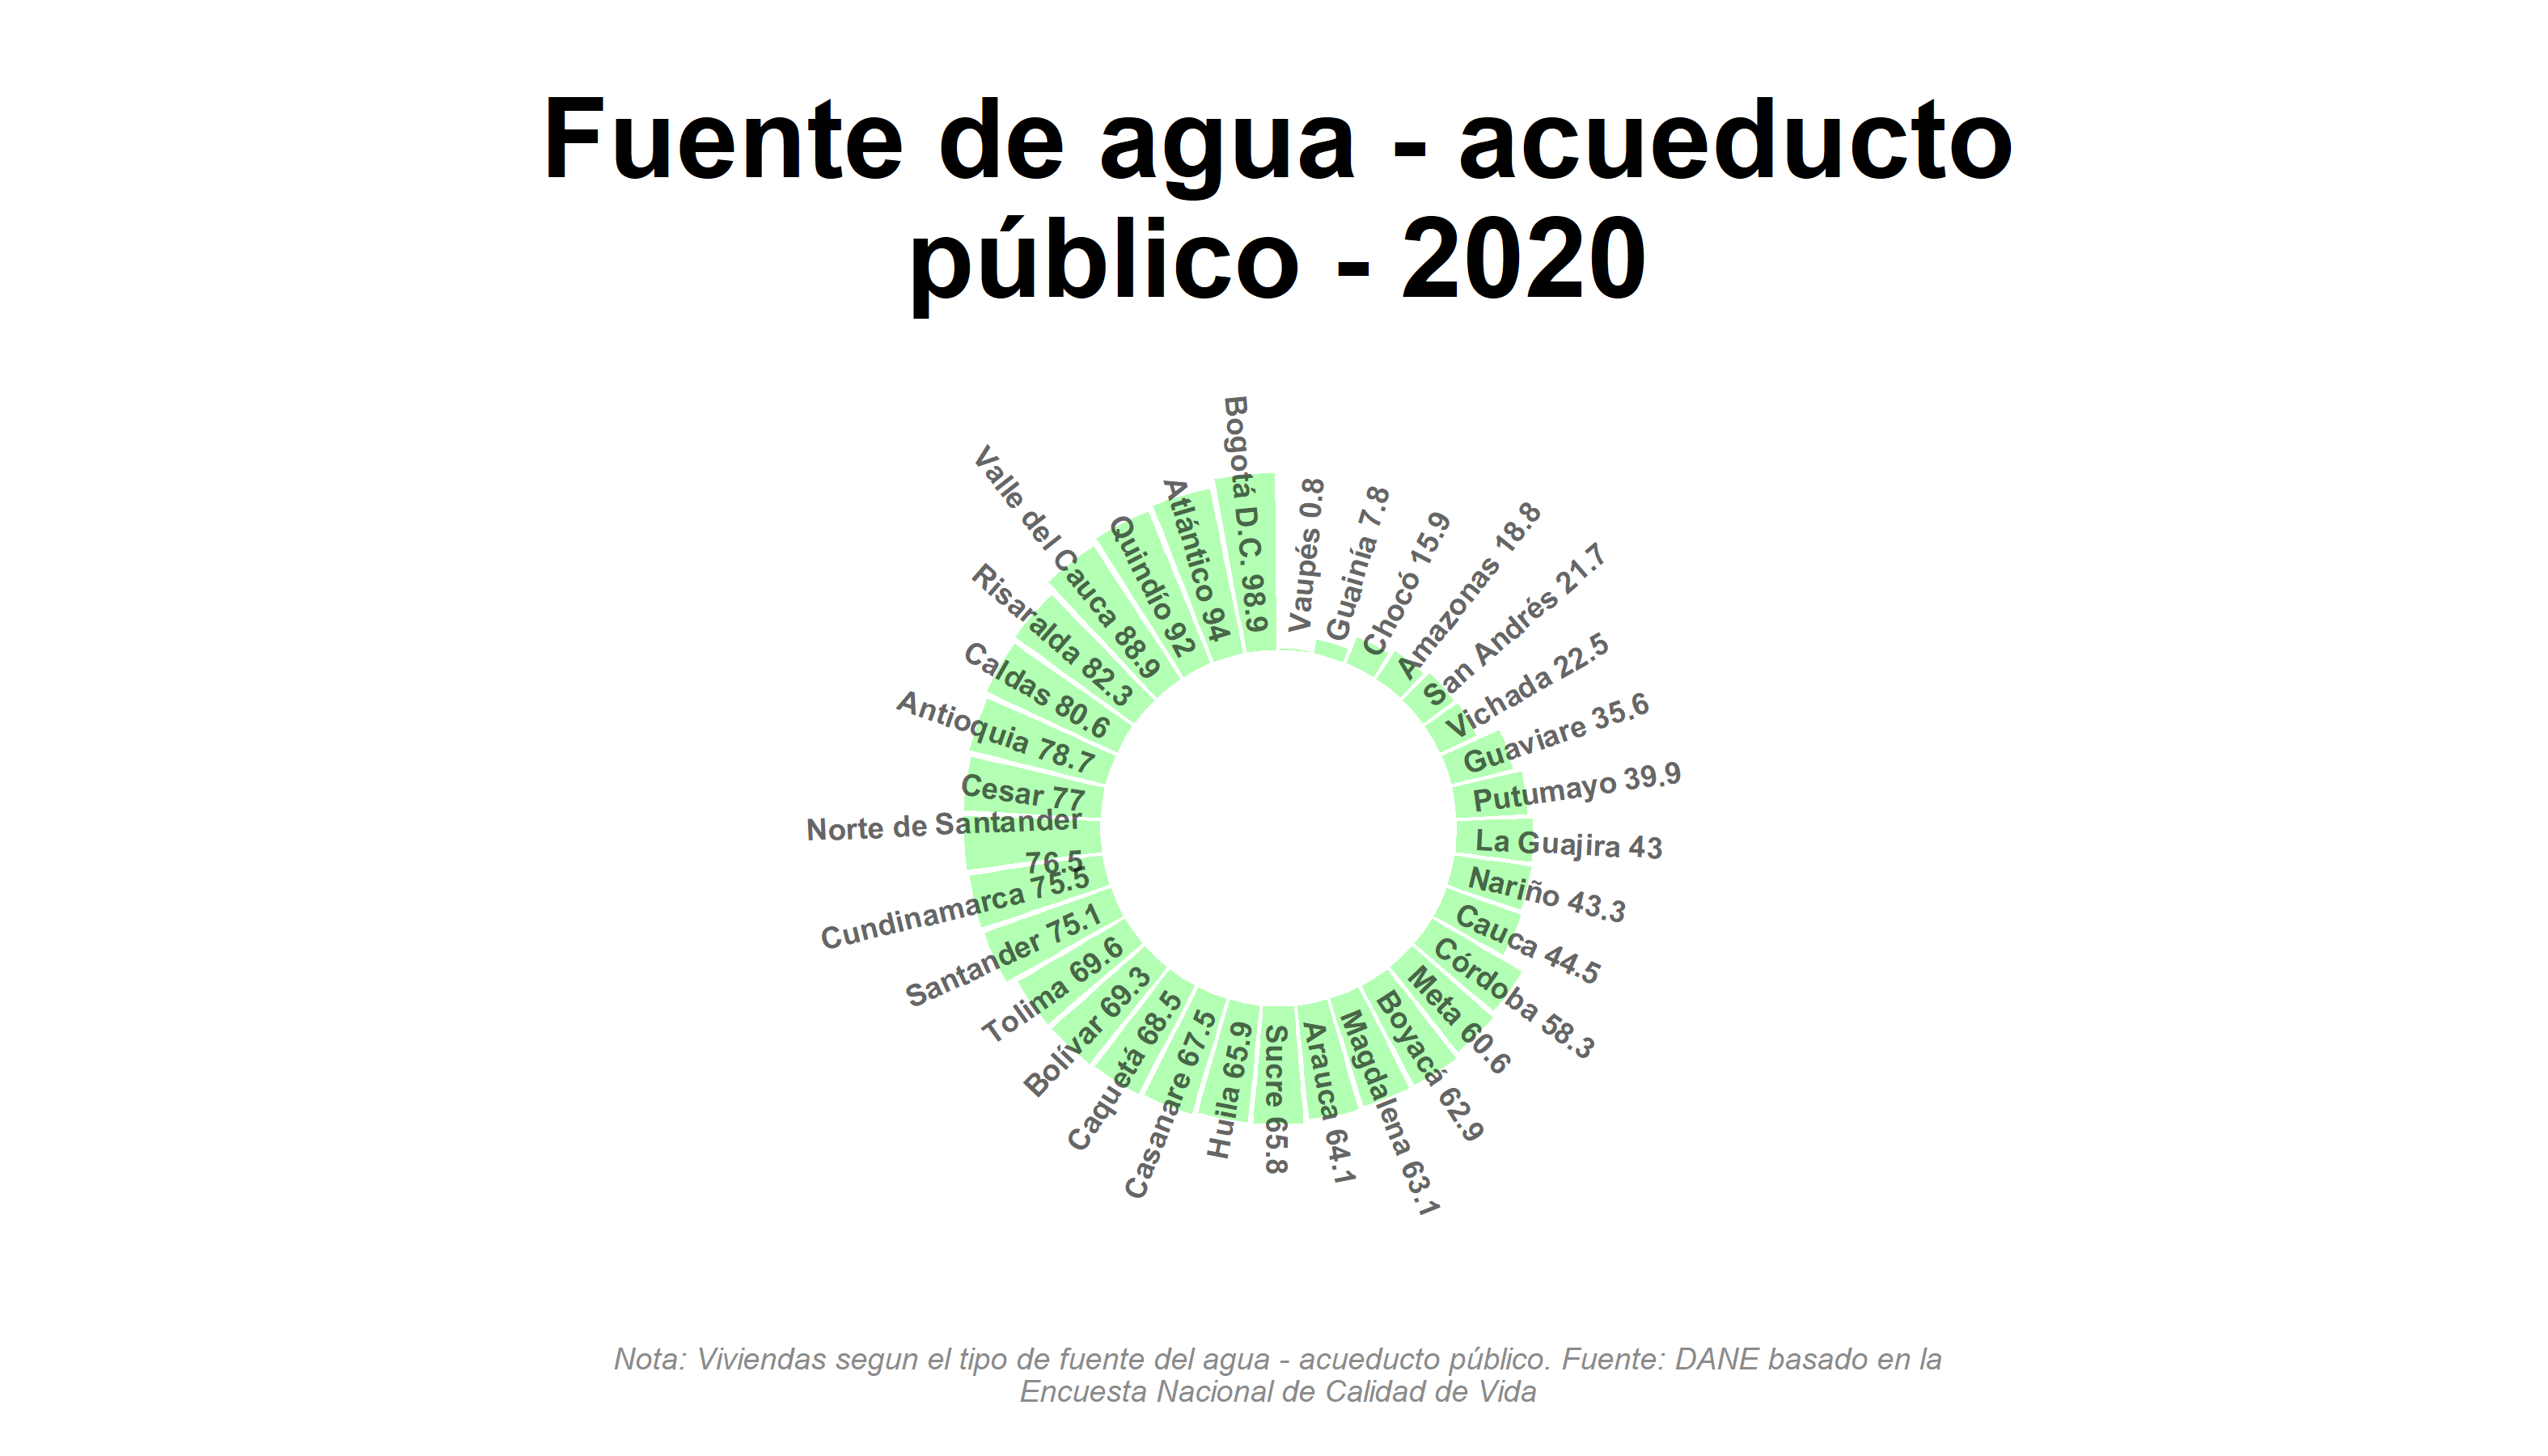
\includegraphics[width=\columnwidth]{img/var_129_static.png}
            \end{imagecolumn}
            \begin{textcolumn}
                \begin{itemize}
                    \item La ocupación de minoría (indígenas, negritudes, ...) en el mercado laboral se caracteriza por su alta informalidad
                \end{itemize}
            \end{textcolumn}
    \printcolumns
    \end{slide}
    
    
    \begin{slide}{15} 
            \begin{imagecolumn}
                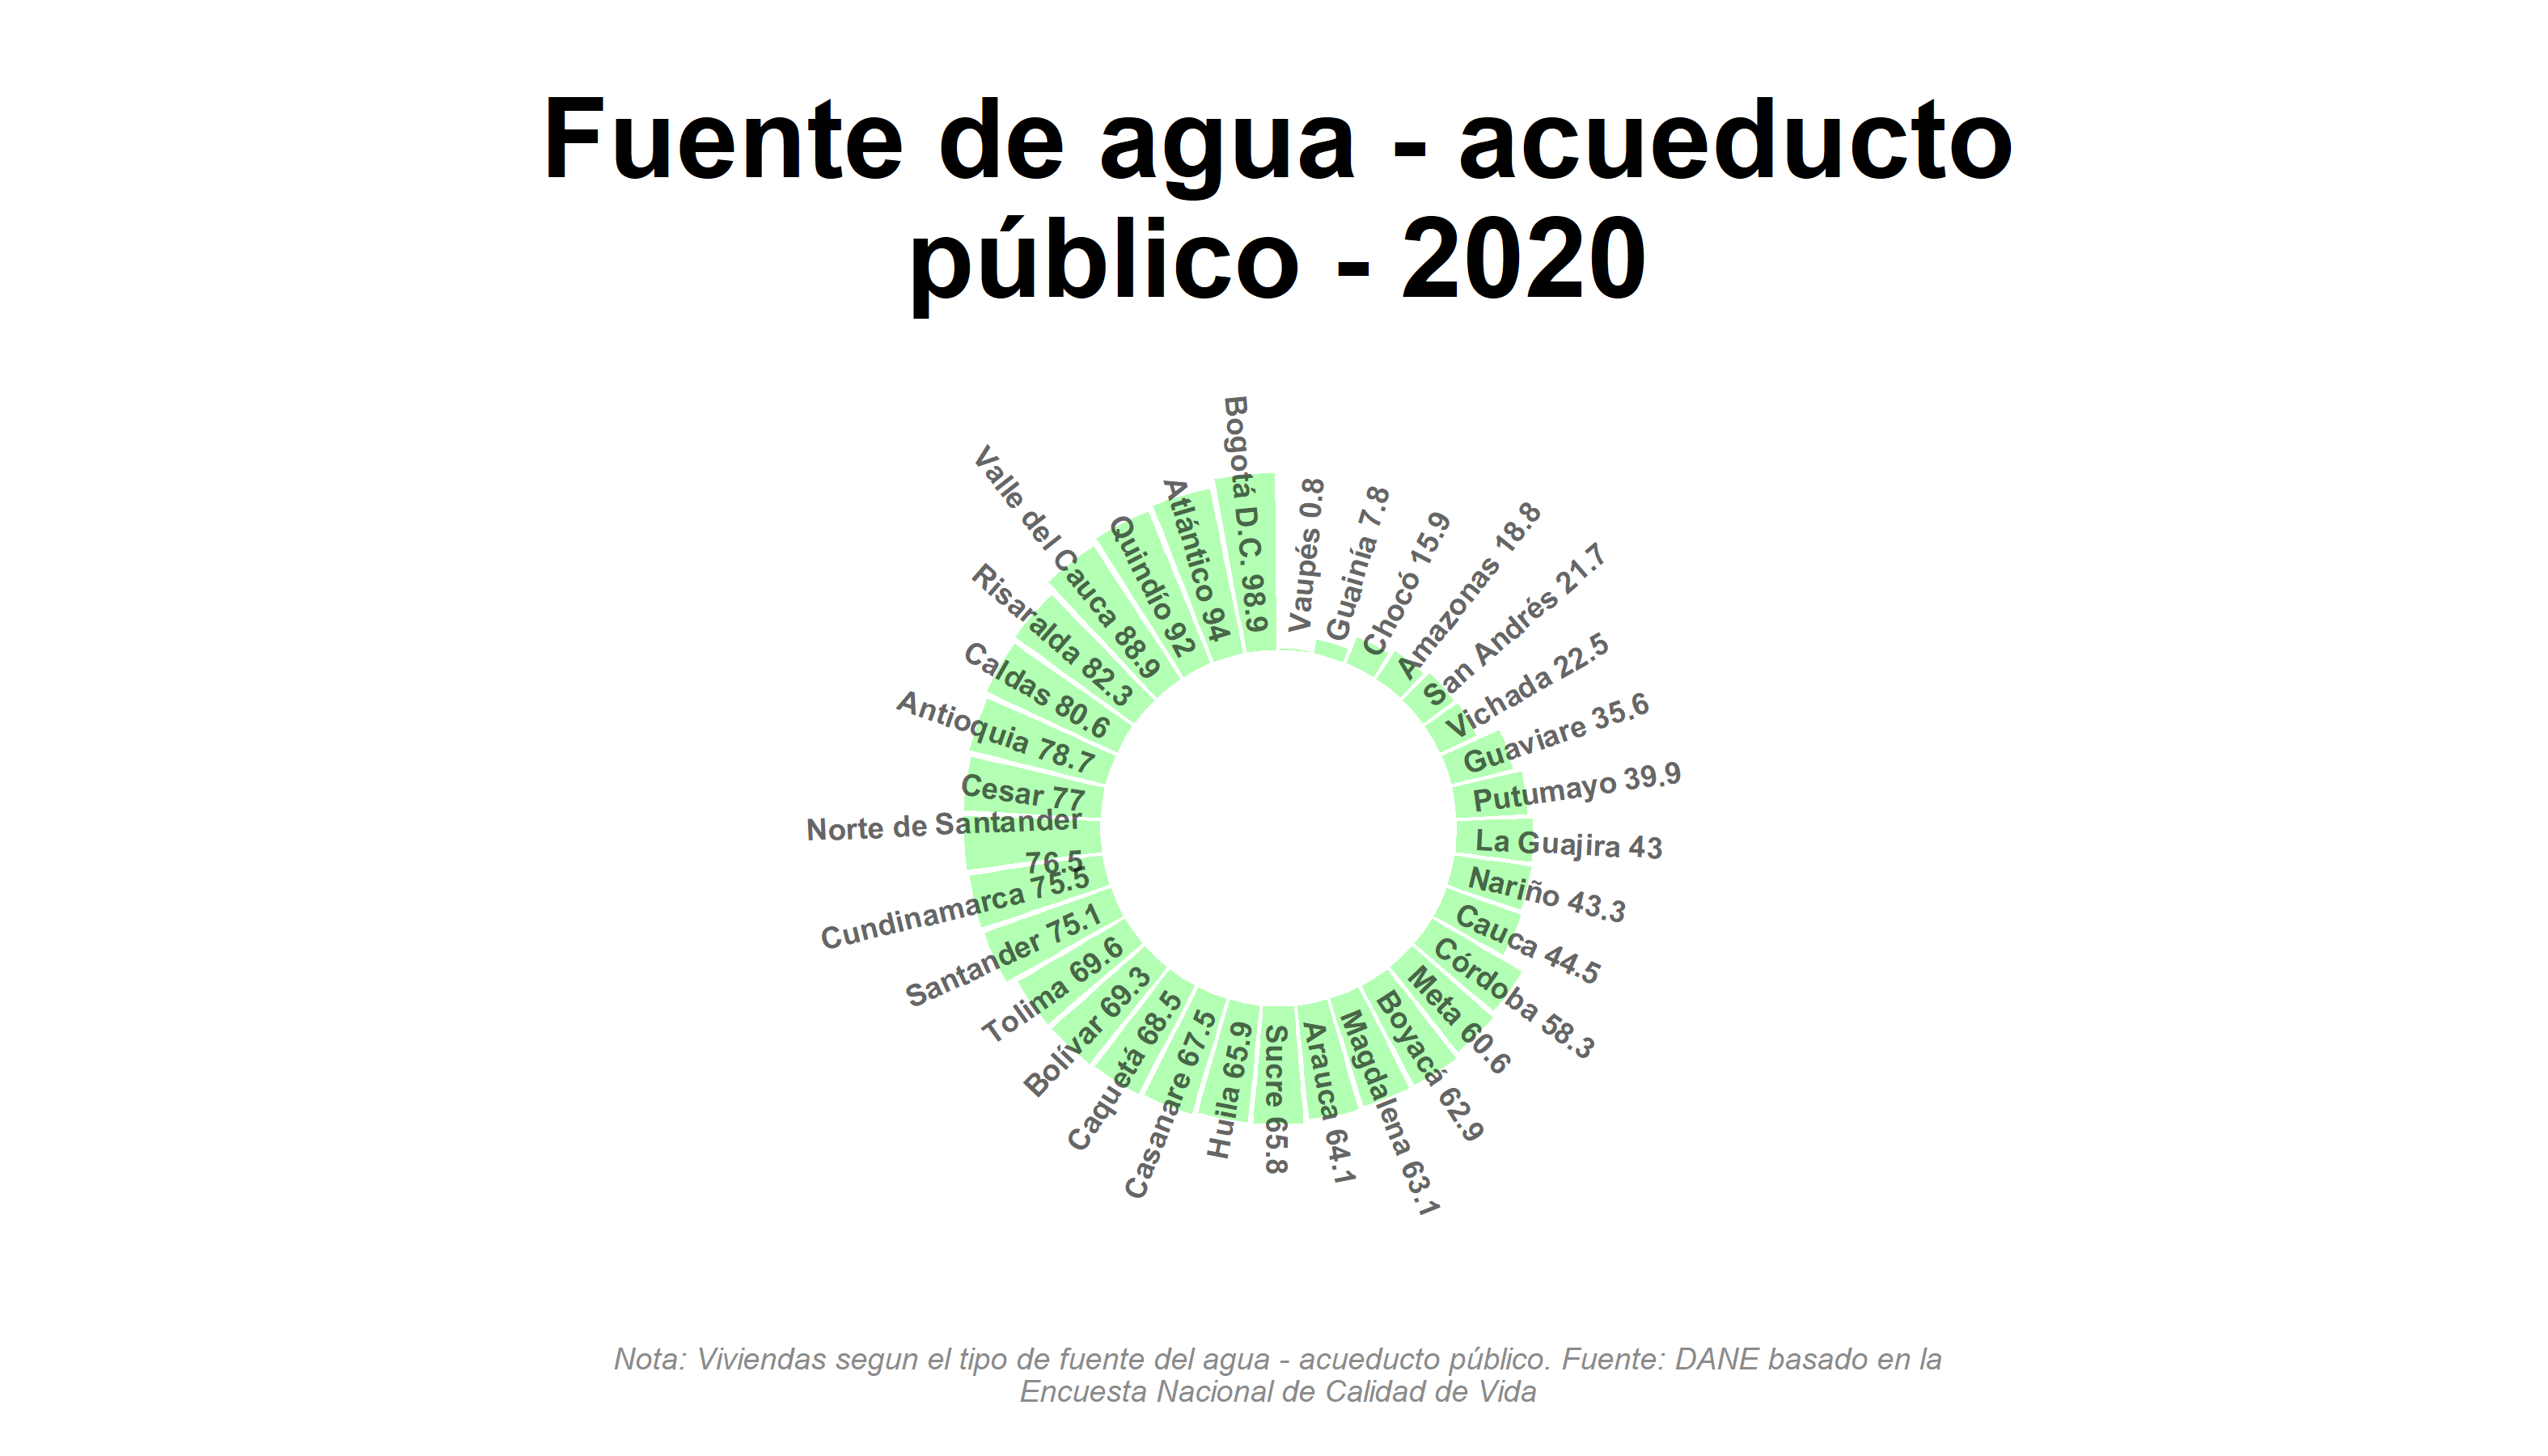
\includegraphics[width=\columnwidth]{img/var_129_static.png}
            \end{imagecolumn}
            \begin{textcolumn}
                \begin{itemize}
                    \item La ocupación de minoría (indígenas, negritudes, ...) en el mercado laboral se caracteriza por su alta informalidad
                \end{itemize}
            \end{textcolumn}
    \printcolumns
    \end{slide}
    
    
        \begin{slide}{15} 
            \begin{imagecolumn}
                \includegraphics[width=\columnwidth]{img/var_387_map.png}
            \end{imagecolumn}
            \begin{textcolumn}
                \begin{itemize}
                    \item Una tendencia a la baja en los homicidios, pero con una alta concentración territorial.
                \end{itemize}
            \end{textcolumn}
    \printcolumns
    \end{slide}
    
    
    
    
    
      %%% ----------------------------
    %%% Cambio Climático
    %%% ----------------------------
    \subsection{Adultez}
    
            %%%-- Highlights 
    \begin{slide}{16} 
            \begin{imagecolumn}
                \includegraphics[width=\columnwidth]{img/var_381_map.png}
            \end{imagecolumn}
            \begin{textcolumn}
                \begin{itemize}
                    \item Un incremento en el desempleo generalizado debido a la pandemia
                    \item Con algunas ciudades donde se ha agudizado en mayor magnitud
                \end{itemize}
            \end{textcolumn}
    \printcolumns
    \end{slide}
    
          %%% ----------------------------
    %%% Cambio Climático
    %%% ----------------------------
      \section{Colombias}
    %%% Contexto
    \slidetitle{17}
    
                %%%-- Highlights 
    \begin{slide}{18} 
            \begin{imagecolumn}
                \includegraphics[width=\columnwidth]{img/mapa_cluster.png}
            \end{imagecolumn}
            \begin{textcolumn}
                \begin{itemize}
                    \item Índice por cada dimensión
                    \item 4 grupos de departamentos
                \end{itemize}
            \end{textcolumn}
    \printcolumns
    \end{slide}
    
        %%% Contexto
    \slidetitle{19}
    
    
   
\end{document}